\documentclass[bigchapter,type=bsc,colorback,accentcolor=tud6d]{tudthesis}

%--------------------------------------------------------
% shows reference keys
%--------------------------------------------------------
%TODO: remove for final
%\usepackage{showkeys}

%--------------------------------------------------------
% provides the todo command
%--------------------------------------------------------
\newcommand\todob[1]{{\color{red}\fbox{
\begin{minipage}{\textwidth-4pt}\texttt{ TODO: #1 }\end{minipage}}}}

\newcommand\todo[1]{{\color{red}\fbox{\texttt{\footnotesize TODO: #1}}}}

%--------------------------------------------------------
% more package references
%--------------------------------------------------------
%\usepackage{ngerman}   ...ist ja gar nicht auf deutsch!
\usepackage{booktabs}
\usepackage{tabularx}

\usepackage{hyperref}

\usepackage{varwidth}

\usepackage{graphicx}
\usepackage{wrapfig}

\usepackage[bibencoding=utf8]{biblatex}
%\usepackage{parskip}

% new page for each section
%\usepackage{titlesec}
%\newcommand{\sectionbreak}{\clearpage}

% flow charts etc.
\usepackage{tikz}
\usetikzlibrary{shapes,arrows,positioning,automata}

\usepackage{listings}
\usepackage{lstlinebgrd}

%--------------------------------------------------------
% configuration
%--------------------------------------------------------

%\bibliographystyle{IEEEtran}
\bibliography{thesis-h2-mptcp}

\setlength{\parskip}{0.75\baselineskip}%
%\setlength{\parindent}{0pt}%

% increase line height
\renewcommand{\baselinestretch}{1.2} 

\newcommand\code[1]{\texttt{\protect\detokenize{#1}}}

% german month for TUDthesis
\newcommand{\getmydate}{%
	\ifcase\month%
	\or Januar\or Februar\or M\"arz%
	\or April\or Mai\or Juni\or Juli%
	\or August\or September\or Oktober%
	\or November\or Dezember%
	\fi\ \number\year%
}

\definecolor{mygreen}{rgb}{0,0.6,0}
\definecolor{mygray}{rgb}{0.5,0.5,0.5}
\definecolor{mymauve}{rgb}{0.58,0,0.82}

\lstset{ %
  escapeinside={(*}{*)},
  basicstyle=\footnotesize\ttfamily,        % the size of the fonts that are used for the code
  breakatwhitespace=false,         % sets if automatic breaks should only happen at whitespace
  breaklines=true,                 % sets automatic line breaking
  captionpos=b,                    % sets the caption-position to bottom
  commentstyle=\color{mygreen},    % comment style
  extendedchars=true,              % lets you use non-ASCII characters; for 8-bits encodings only, does not work with UTF-8
  frame=single,	                   % adds a frame around the code
  keepspaces=true,                 % keeps spaces in text, useful for keeping indentation of code (possibly needs columns=flexible)
  keywordstyle=\color{blue},       % keyword style
  %numbers=left,                    % where to put the line-numbers; possible values are (none, left, right)
  %numbersep=5pt,                   % how far the line-numbers are from the code
  %numberstyle=\tiny\color{mygray}, % the style that is used for the line-numbers
  rulecolor=\color{black},         % if not set, the frame-color may be changed on line-breaks within not-black text (e.g. comments (green here))
  showspaces=false,                % show spaces everywhere adding particular underscores; it overrides 'showstringspaces'
  showstringspaces=false,          % underline spaces within strings only
  showtabs=false,                  % show tabs within strings adding particular underscores
  %stepnumber=2,                    % the step between two line-numbers. If it's 1, each line will be numbered
  stringstyle=\color{mymauve},     % string literal style
  tabsize=2,	                   % sets default tabsize to 2 spaces
  title=\lstname                   % show the filename of files included with \lstinputlisting; also try caption instead of title
}
\lstdefinestyle{RBS}{
  language=C,                 % the language of the code
  morekeywords={SCHEDULER,VAR,IF,ELSE,FOREACH,RETURN,SET,IN}           % if you want to add more keywords to the set
}

\lstdefinestyle{C_Code}{
  language=C                 % the language of the code
}


\makeatletter
%%%%%%%%%%%%%%%%%%%%%%%%%%%%%%%%%%%%%%%%%%%%%%%%%%%%%%%%%%%%%%%%%%%%%%%%%%%%%%
%
% \btIfInRange{number}{range list}{TRUE}{FALSE}
%
% Test in int number <number> is element of a (comma separated) list of ranges
% (such as: {1,3-5,7,10-12,14}) and processes <TRUE> or <FALSE> respectively

\newcount\bt@rangea
\newcount\bt@rangeb

\newcommand\btIfInRange[2]{%
    \global\let\bt@inrange\@secondoftwo%
    \edef\bt@rangelist{#2}%
    \foreach \range in \bt@rangelist {%
        \afterassignment\bt@getrangeb%
        \bt@rangea=0\range\relax%
        \pgfmathtruncatemacro\result{ ( #1 >= \bt@rangea) && (#1 <= \bt@rangeb) }%
        \ifnum\result=1\relax%
            \breakforeach%
            \global\let\bt@inrange\@firstoftwo%
        \fi%
    }%
    \bt@inrange%
}
\newcommand\bt@getrangeb{%
    \@ifnextchar\relax%
        {\bt@rangeb=\bt@rangea}%
        {\@getrangeb}%
}
\def\@getrangeb-#1\relax{%
    \ifx\relax#1\relax%
        \bt@rangeb=100000%   \maxdimen is too large for pgfmath
    \else%
        \bt@rangeb=#1\relax%
    \fi%
}


%%%%%%%%%%%%%%%%%%%%%%%%%%%%%%%%%%%%%%%%%%%%%%%%%%%%%%%%%%%%%%%%%%%%%%%%%%%%%%
%
% \lstHighlightRange{range list}
%
% Highlights lines in range list in a lstlisting linebackgroundcolor parameter
\definecolor{codehladded}{HTML}{EAFFEA}
\definecolor{codehlremoved}{HTML}{FFECEC}
\definecolor{codehlhighlight}{HTML}{FFF9E8}

\newcommand\lstLinesAdded[1]{\btIfInRange{\value{lstnumber}}{#1}{\color{codehladded}}{}}
\newcommand\lstLinesRemoved[1]{\btIfInRange{\value{lstnumber}}{#1}{\color{codehlremoved}}{}}
\newcommand\lstLinesHighlight[1]{\btIfInRange{\value{lstnumber}}{#1}{\color{codehlhighlight}}{}}

\makeatother

%=================================================================================
% start of document
%=================================================================================

\begin{document}




%=====================================================================
% Title Page
%=====================================================================

\thesistitle{Optimierte Zusammenarbeit von HTTP/2 und Multipath TCP}{Optimizing Cooperation of HTTP/2 and Multipath TCP}
\author{Maxi Weller}
\referee{Prof. Ralf Steinmetz}{Alexander Fr�mmgen}
\department{Fachbereich Informatik}
\group{Multimedia Communications Lab }
\tuprints{57580}{5758}
\makethesistitle
\affidavit{M. Weller}


%=====================================================================
\begin{abstract}
%=====================================================================

Multipath TCP is an extension to the Transmission Control Protocol (TCP) to support the use of multiple paths between hosts with multiple interfaces. An implementation of Multipath TCP has to decide for each data segment over which path it should be sent. This decision can be based on different criteria and algorithms, making a trade-off between throughput, resource utilization, reliability and latency. Multipath TCP is backwards compatible to TCP, not only on the wire, but also towards the application layer. With the current reference implementations, applications do not have to be aware of Multipath TCP, but they also can't influence the scheduling decisions.
 %\cite{RFC6182}

We show that hints from the application can improve scheduling performance. We enable the application to select and modify the scheduling algorithm based on its internal information about content types, priorities, dependencies and user expectations.
For this, we modify an HTTP/2 web server to pass scheduling hints to the Multipath TCP scheduler via socket options. The scheduling algorithms are developed in the RBS scripting language for easier evaluation.
An evaluation is performed in simulated and real-world environments over LTE and WiFi.


\end{abstract}

%MPTCP-Implementierungen m�ssen f�r jedes Datensegment entscheiden, �ber welchen Pfad es gesendet werden soll. Diese Entscheidung kann auf unterschiedlichen Kriterien und Algorithmen basieren, wobei zwischen Durchsatz, Ressourcennutzung, Zuverl�ssigkeit und Latenz abgew�gt wird. 
%MPTCP ist vollst�ndig abw�rtskompatibel zur Anwendungsschicht. Daher hat die Anwendung normalerweise keinen Einfluss auf diese Abw�gung, obwohl sie �ber zus�tzliche Informationen verf�gt. 


%=====================================================================
\renewcommand{\contentsname}{Contents}
%=====================================================================

\tableofcontents

\listoffigures

\listoftables

\lstlistoflistings


%=====================================================================
\chapter{Introduction}
%=====================================================================

In the following paragraphs, we describe the motivation for the relatively recent protocols this work is based on as well as for the kind of optimizations that will be implemented in this thesis. We introduce the approach and give an overview of the remaining chapters.






%---------------------------------------------------------------------
\section{Motivation}
%---------------------------------------------------------------------

\begin{wrapfigure}{r}{0.45\textwidth}
	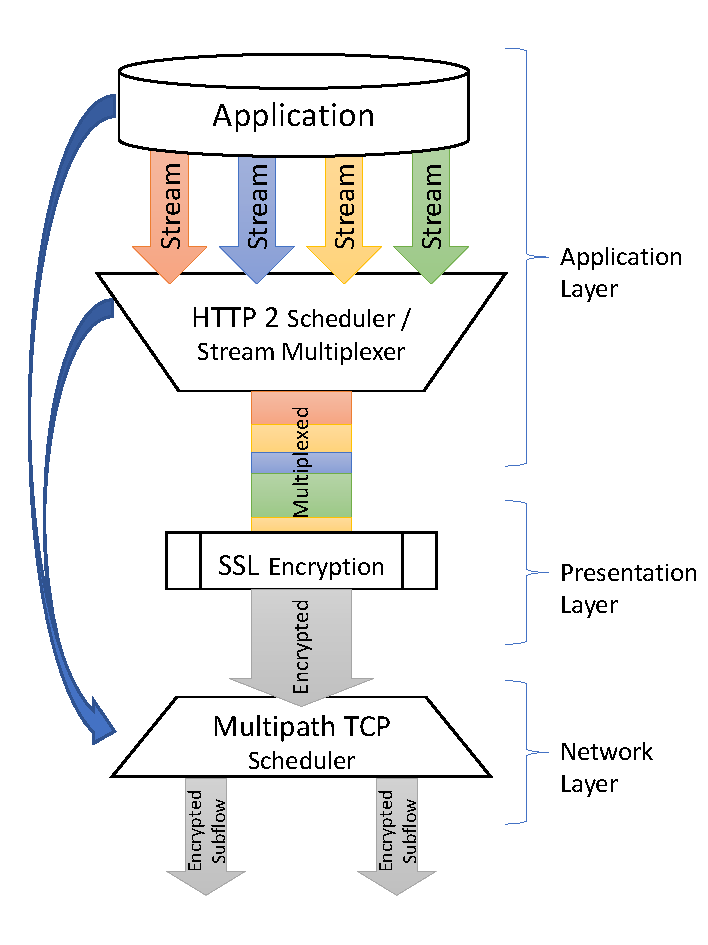
\includegraphics[width=0.4\textwidth]{mux-demux.pdf}
	\caption{Optimization across layers}
\end{wrapfigure}


% reasoning why mptcp is/will be used on devices people browse the internet with
Most smart phones and notebooks have multiple network interfaces nowadays. This has given rise to the design of various network protocols with the aim of extending bandwidth, enhancing reliability and lowering power consumption by intelligently combining interfaces. One of these is Multipath TCP  \cite{RFC6824_MPTCP}, an extension to the Transmission Control Protocol with support for combining multiple paths over multiple interfaces into a single TCP connection with higher bandwidth and reliability.


% users expect faster/instant reaction from computers/web pages/interactive services ^= do not accept (long) wait times
% web sites getting more complex
% 
% very short intro to mptcp, evtl. richtung vorteile f�r clients/webbrowsing
% ``more and more devices are mobile''
% ``almost every modern device has multiple network interfaces'' (smartphones cell+wifi, notebooks eth+wifi(+cell), desktops eth+wifi, household routers with multi uplink dsl+lte, etc)



Inherent in Multipath TCP operation is some overhead of discovering and establishing multiple paths when the connection is set up. In regular web browsing, HTTP up to version 1.1 use many short-lived TCP connections, so the overhead of multipath initialization can shatter the performance improvements of Multipath TCP, as the connection often is closed before the second path is usable. Combined with unadapted browsers, this can cause Multipath TCP to have worse performance than single path TCP \cite{han2015mwebmptcp}.


% very short intro to http/2, maybe difference to http/1(.1)
% ``websites become more intricate''
The web has come a long way since the introduction of HTTP/0.9 in 1993. Many small improvements have been made in the meantime, all carefully providing backward compatibility. But web applications have become so intricate, and users so accustomed to responsive interactive services, that a clear break had to be made. Therefore, HTTP/2 \cite{RFC7540_HTTP2} has been specified. To allow easier adaption, the semantics were kept intact, while the underlying protocol was changed completely: A only seemingly simple text-based protocol was replaced with a more efficient, precisely specified binary protocol. 
The new feature most relevant to us are multiplexed streams which allow all data to be transferred over few, long-lived, thus more efficient TCP connections. The multiplexing also prevents head-of-line blocking and allows prioritizing the most time-critical resources.

% two schedulers (
% - http2 schedules frames from multiple streams into one tls/tcp connection, mostly based on http2 priority;
% - mptcp schedules tcp segments from one meta socket onto multiple real sockets
% )
% three layers

As opposed to older versions, HTTP/2 is based on long-lived TCP connections. Therefore it can utilize the additional sub-flow capacity more often. During a single connection, different types of requests are processed, including loading a document and resources required to display it, loading auxiliary content like images below the fold, and user-initiated AJAX requests. Every type of request has different performance needs, which makes it especially interesting for cooperation-based optimization approaches.

% different scheduling approaches for mptcp are possible, many have been proposed and some are implemented in the linux kernel

% assumption: choosing best possible scheduling strategy depends on requirements of(/knowledge about/knowledge available to implementation of) higher level protocols 
% even for one given protocol, these requirements can change during a connection (e.g. web site: initial loading should be fast - user is waiting - use fastest flow(s)/use redundancy, loading of images below the fold don't need to be as fast -> conserve power/metered traffic, ajax requests might be small, but latency critical -> redundancy)
We assume that choosing the best possible Multipath TCP subflow scheduling strategy depends on information about the higher layers. In the case of HTTP/2 connections this information includes the type of the request as indicated above. For having this information available to the packet scheduler - part of the transport layer - there are several possible solutions, each coming with different pros and cons. 
% for some protocols, a good heuristical approach can be chosen based on transmitted bytes, time, transmission pauses, etc
For one, a heuristic approach can be chosen, which acts on metadata readily available in the transport layer, including transmission rate and pauses, elapsed time, and byte and packet counters. The good thing is that this approach is independent of the specific implementation of the application protocol, and can even work unchanged for several similar protocols. 
% for some protocols, the scheduler could look into the octet stream and decide depending on contents
% problems:
% -> breaks separation of layers - high ``dirty hack'' factor
% -> protocol decoding needs to be implemented in scheduler (os kernel!) -> proto updates need kernel updates, security problems (protocol parser is huge attack surface)
% -> impossible with encrypted protocols (not technically impossible, but would be very complicated and has performance hit)
Even more information about the state of higher level protocols can be gained by inspecting the octet stream itself. This brings with it all problems of Deep Packet Inspection, including security risks and increased code complexity \cite{Porter2005}. It is also not applicable to HTTP/2 as all browsers implement it with forced TLS encryption, therefore this approach is not considered any further.
% solution / our approach: the implementation of the higher level protocol provides special scheduling hints to the mptcp scheduler
% pro
% - no detailed knowledge about the protocol is neccessary in the scheduler
% - with a good api, the scheduler needs to know nothing about the specific application level protocol, while the app level proto implementation needs to know (almost) nothing about the network level scheduling
% contra
% - every application which should take advantage of this approach needs to be specifically modified
% - 
The middle road we suggest is providing an API which allows the application to provide scheduling hints to the transport layer. This has the advantage of not embedding knowledge about the application layer protocol in the scheduler, thereby keeping the abstraction layers separate.


%---------------------------------------------------------------------
\section{Approach}
%---------------------------------------------------------------------

%\todob{conceptual approach}
%wie vorgehen - konzeptioneller approach
%interaction / dependency -> l�sen durch cooperation
We start by analyzing the general structure of popular web sites regarding the resources on the critical path. In comparison, we look at guidelines for performance optimization in web design. 
From the gained insights, we conceive possible optimizations for existing, modified or specially crafted web pages at the transport level. The Multipath TCP implementation \cite{multipathtcp} consists of three major building blocks: path manager, packet scheduler and connection to the subflows \cite{RFC6182}. In this thesis, we pay special attention to the packet scheduler. More precisely, we concentrate on its component which spreads individual segments over subflows. These optimized schedulers are implemented in rule-based scripts which are loaded into the MPTCP implementation in the Linux kernel. To make scheduling hints like content type, priorities or dependencies available to the scheduler scripts, we modify a suitable HTTP/2-capable web server to pass on these hints as socket options. 

%auch implement. und eval approach
The next step is an evaluation of the implemented optimizations in simulated network environments. Web sites are loaded in network scenarios differing in bandwidth, round trip time and packet loss. To study the practicality, we conduct real-world measurements for the best-performing optimizations, connecting from LTE and domestic ADSL access networks to virtual servers at a cloud provider. 



%


%---------------------------------------------------------------------
\section{Structure}
%---------------------------------------------------------------------
% where we provide an overview of the chapters

% background/rel. work
In the following chapter, we introduce the protocols on which this work is based. This is Multipath TCP on the transport layer, which is described with a focus on scheduling. On the application layer, the HTTP/2 protocol and its underlying concepts. A review of related publications is conducted, with a focus on  Multipath TCP scheduling, coordination among software layers, cooperation between kernel and user-space components, web page optimization, and performance measurement of web pages and applications.

%approach
Chapter four starts with an analysis of typical web page structures, details our approach for passing scheduling hints from application to transport layer and presents optimized MPTCP scheduler rules for different network scenarios. We also consider security concerns regarding the scheduling hints as a side channel to TLS encryption.

%implementation
Following our approach of integrating multiple layers, the implementation described in chapter five ranges from the network layer up to the application layer. Optimized schedulers were realized with a scripting-enabled rule based scheduler in the Linux kernel. After conducting a survey of web server software, we choose one to customize. This is necessary to pass information about HTTP transactions down the stack, bypassing encryption. On top of that, we created sample web pages and applications.


%evaluation
To show which optimizations are worth using in which network situations, in chapter five, we evaluate the performance of the implemented schedulers in simulated and real-world networks. We conduct measurements including the resource usage, like transmitted data volume per interface, and record timestamps of all events in the browser, to calculate various page load speed metrics. Based on that data, we relate the added value for the user to potential computational overhead and bandwidth costs.


%their actual and perceived speed, utility to the user, overall and per-interface bandwidth usage, (power usage?), computational overhead, implementation difficulty, 

%conclusion
Finally, a conclusion is drawn on the accomplished improvements, which approaches were successful and which less so. We also use the last chapter to point out possible future work.


%problem statement

% analysis of the possible ways for interaction between transport and application layer in the case of MPTCP and HTTP2

% analysis of typical web page structures

% design and implementation of MPTCP scheduler(s) for optimizing web page loading / web app usage, which get (out of band) information from presentation layer TLS, application layer HTTP2 and/or  application layer HTML, JS,... (Web Page Structure)

% evaluation of the optimizations





%=====================================================================
\chapter{Background and Related Work}
%=====================================================================

%related work
In this chapter, we go through transport, presentation and application layer, the OSI layers this work is concerned with. For each layer, we explain the relevant protocols and implementations. We will also present previous work on the optimization and measurement of web page performance.


\section{Transport Layer: Multipath TCP}


\begin{figure}
	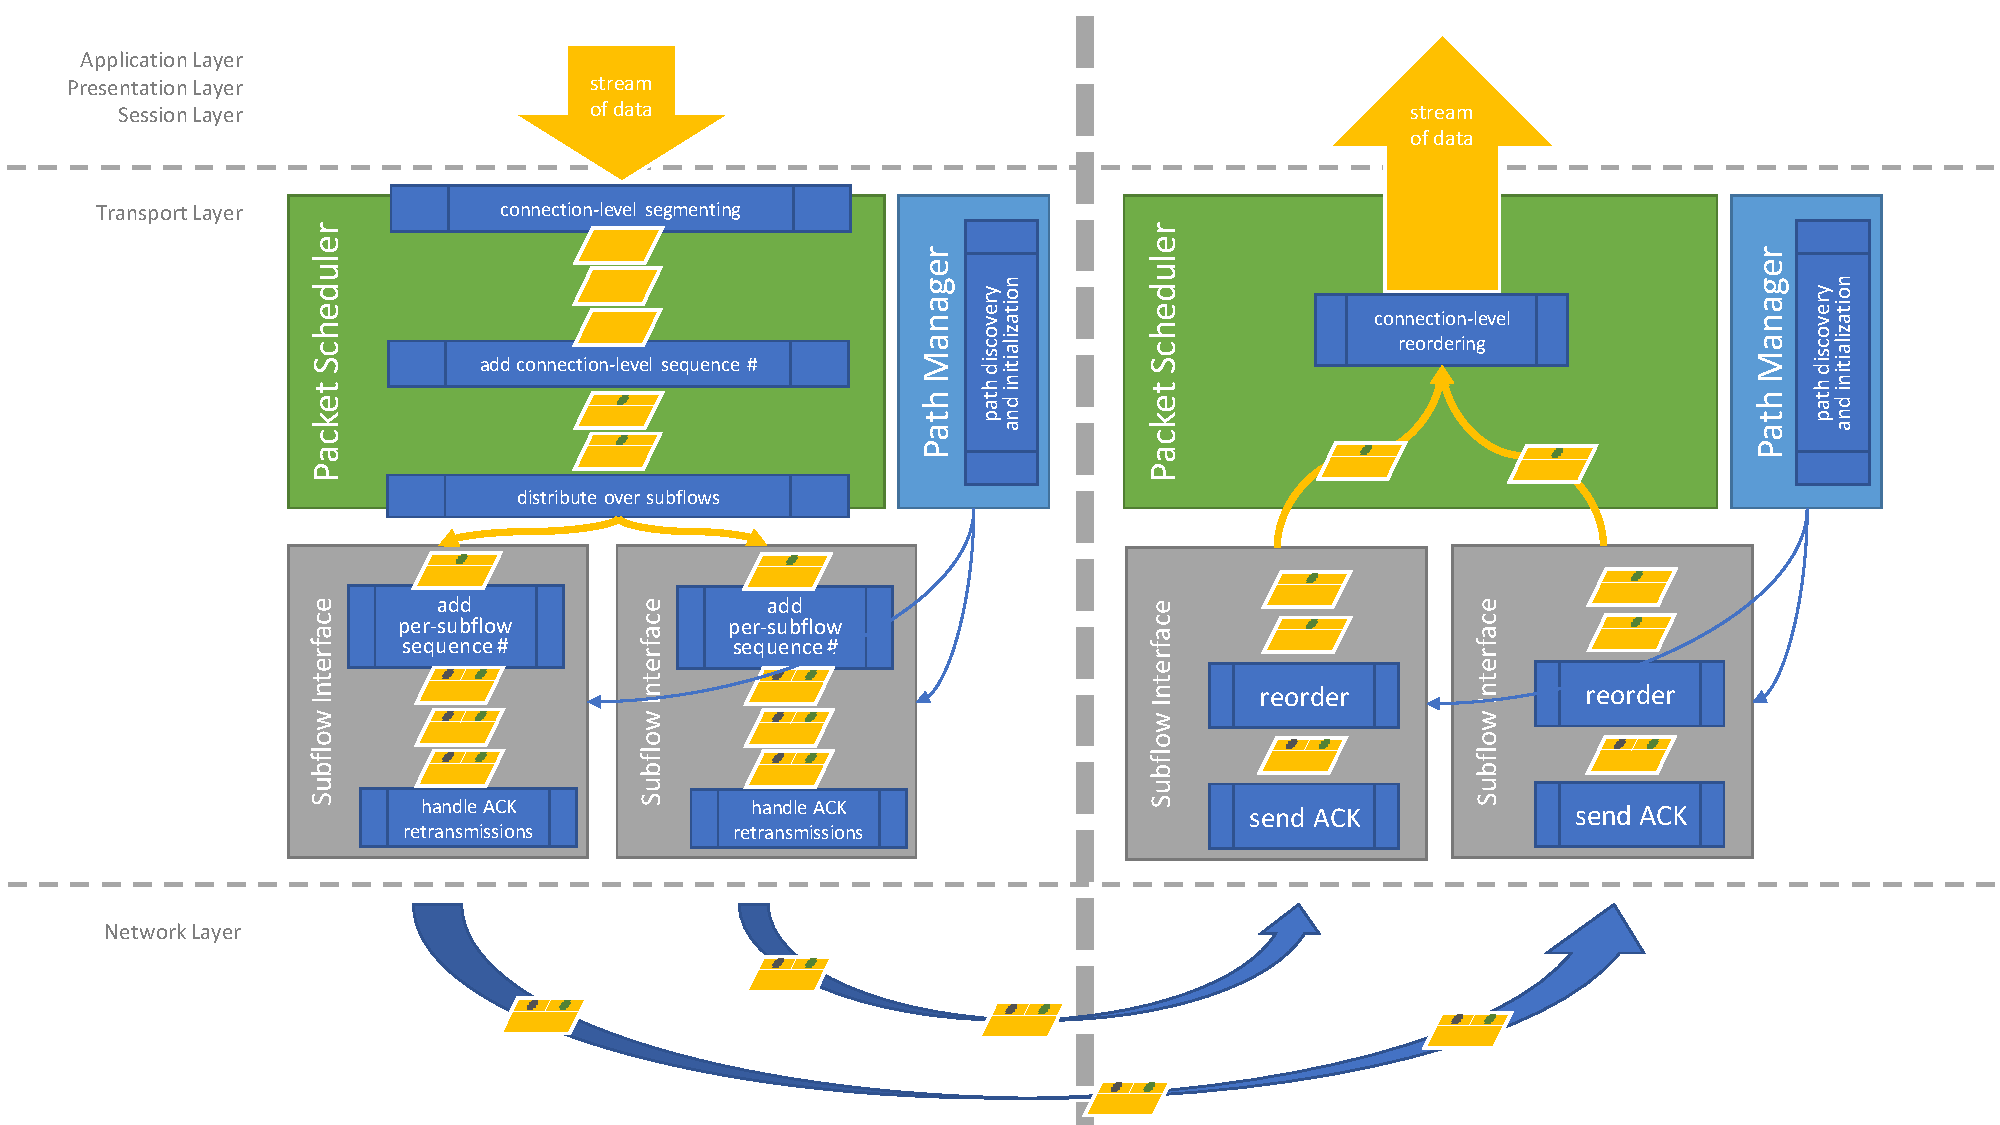
\includegraphics[width=1\textwidth]{mptcp-functional-decomposition.pdf}
	\caption{Interaction of the functional building blocks of Multipath TCP as described in \cite{RFC6182}}
\end{figure}
%
%http://www.ip-insider.de/anwendungen-und-konkurrenz-fuer-multipath-tcp-a-445245/
%

Two pipes are better than one - that's Multipath TCP in a nutshell \cite{IpInsiderMptcp}. In this case, a pipe is a distinct path between two devices, identified by the IP adresses of both peers. Combining multiple of these subflows can provide several advantages. Higher throughput can be achieved by multiplexing data over multiple subflows. The reliability of a connection can be improved by establishing backup subflows: in case a subflow stops working, the backup takes over seamlessly. On routes with packet loss, the latency can be reduced by sending packets redundantly on multiple subflows.

This section covers the background knowledge on Multipath TCP which is required for the remaining work. We start by enumerating the current software implementations of Multipath TCP and giving some information on its current deployment. Following that, we describe the architecture of protocol and implementations. We present studies evaluating and optimizing Multipath TCP performance, and proposals and implementions of interfaces to the application layer. To finish this section, we explain the rule-based scheduler, a Multipath TCP packet scheduler, which makes its decisions based on script programs which are changeable during runtime, allowing us to evaluate different scheduling approaches faster.

%tuple of (source address, source port, destination address, destination port).




\subsection{Implementations and Deployment}
%We start by enumerating the current software implementations of Multipath TCP and giving some information on its current deployment.

%reference(?) implementation in linux kernel
The current reference implementation\footnote{\url{http://multipath-tcp.org/}} is based on the Linux kernel and maintained by \textcite{multipathtcp} at the Universit� Catholique de Louvain. A similar patch for the FreeBSD kernel has been developed at Swinburne University\footnote{\url{http://caia.swin.edu.au/newtcp/mptcp/}}.
%https://support.apple.com/en-us/HT201373
 The first implementation of Multipath TCP was developed as a user-space proxy\footnote{\url{https://open-innovation.alcatel-lucent.com/projects/mptcp-proxy}} by Hampel at Bell Labs, and is no longer maintained.  
%other implementations
The most widely deployed implementation is found in Apple's XNU kernel \cite{Hesmans2016}, used in the macOS and iOS operating systems. It is used mainly for the Siri personal assistant software, which keeps a backup connection over cellular network in case the Wi-Fi connection breaks down \cite{AppleSupportMPTCP}. 
All aforementioned implementations are open source. There is also one known closed-source implementation by Citrix Networks in their load balancer firmware \cite{Eardley2013}.

\textcite{Bonaventure2016Deploy} report a deployment by some cellular network 
operators. Hardware vendors include the Multipath TCP implementation in the 
Linux kernel of their Android phones. The cellular provider provides a SOCKS 
proxy server at carrier level. Together with a SOCKS proxy in the Android 
operating system, both using Multipath TCP, this allows combining Wi-Fi and 
cellular connectivity over existing infrastructure. 
They also describe a deployment scenario where customers of ``hybrid access 
networks'' are connected over DSL and wireless links, which are combined 
using Multipath TCP to achieve higher bandwidth.
In general, Multipath TCP can be deployed in scenarios where at least one peer 
has multiple interfaces. This is the case for an increasing number of device 
classes, as listed in Table \ref{table:typical-netifs}. In this work, we will 
concentrate on consumer devices with Wi-Fi and cellular interfaces.

% multiple network interfaces
\begin{table}%
		\begin{tabular}{ll} \toprule
		Device Type    & Network Interfaces \\ \midrule
		smart phones & Wi-Fi and cellular \\
		notebooks & Wi-Fi, often Ethernet, sometimes cellular \\
		desktops & Ethernet and/or Wi-Fi \\
		servers & multiple Ethernet \\
		household routers with multiple uplinks & DSL and cellular (LTE) \\ \bottomrule
		\end{tabular}
		\caption{Typical network interfaces of common device types}
		\label{table:typical-netifs}
\end{table}


\subsection{Architecture of Multipath TCP}
%Following that, we describe the architecture of the Multipath TCP protocol and implementation. 

\todo{Following that, we describe the architecture of the Multipath TCP protocol and implementation. }


%\subsubsection{Path Management}



%\subsubsection{Packet Scheduling}




%\subsubsection{TCP Subflows}


\subsection{Multipath TCP on the Wire}

Great care was taken in the specification of Multipath TCP to maintain compatibility with regular TCP, not only but especially towards the network layer. This was done with regard to the deploying it in the current Internet, which means coping with network address translators, firewalls and other middleboxes.
Therefore, Multipath TCP subflows look and behave on the wire exactly like regular TCP flows, except the segments contain some additional TCP options as described in RFC 6824 \cite{RFC6824_MPTCP}.

When a new Multipath TCP connection is set up, the \textbf{MP\_CAPABLE} option is included in the SYN segment. From this options, the server learns that the new client supports MPTCP. In the responding SYN-ACK and ACK segments, the MP\_CAPABLE option is included as well, serving as a handshake, in which authentication keys are exchanged. These keys are later used in the process of adding more subflows to the connection.

New subflows are initiated by establishing what looks like a regular TCP connection at to the network, but contains the \textbf{MP\_JOIN} option in the three-way handshake segments. The contents of this option depends on the stage of the handshake. The initiator sends an identifying token, which is based on the authentication keys.  In the first two segments, random numbers (nonces) are exchanged. To authenticate each other, the peers exchange HMACs of the concatenated nonces keyed on the concatenated authentication keys in the second and third segment.

During the regular data transmission, the \textbf{DSS} option (Data Sequence Signal) is added to every segment. It contains sequence numbers and acknowledgements, which work very similar to their TCP counterparts. They are necessary to ensure ordered data transfer across subflows, and to retransmit segments in case of collapse of a subflow.


\subsection{Performance Evaluations}
%We present studies evaluating and optimizing Multipath TCP performance, [...]

\todo{We present studies evaluating and optimizing Multipath TCP performance, [...]}


\subsection{Socket API}
%We present [...] proposals and implementions of interfaces to the application layer.

%application api's
The only way to control the current Linux implementation from user-space was by setting \code{sysctl} parameters, which are generally valid for the entire operating system. They allow the system administrator to enable or disable Multipath TCP for all applications, and to change a number of high-level parameters globally. If Multipath TCP is enabled, it is used for all TCP connections and is transparent to the application. Recently, the socket option \code{MPTCP_ENABLED} was introduced, which allows switching it on or off per socket. Still, application developers don't have any fine-grained control over the Multipath TCP behaviour.

In contrast, the Apple implementation takes a very different approach by providing a new socket-based API. One the positive side, this gives Multipath TCP aware applications full control over Multipath TCP connections, setting up, enumerating and tearing down subflows. New \code{connectx} and \code{disconnectx} system calls are introduced for that reason. However, this makes it incompatible to existing applications, requiring developers to make modifications to take advantage of the new protocol.

To allow similar fine-grained control, while keeping the compatibility with unadapted applications, several APIs have been proposed. 
%RFC 6897
\textcite{Scharf2013} present in RFC 6897 a ``Basic API for MPTCP-Aware Applications'', enabling applications to restrict the interfaces to use for establishing paths and to query the subflows and their addresses. 
They also recommend that socket options on a Multipath TCP meta-socket should be, if possible, passed through to all subflow sockets.
%Hesmans 2016 - An enhanced socket API for Multipath TCP




\subsection{Optimizing Multipath TCP Scheduling}

\todo{?????}


\subsection{Rule-Based Scheduler}
The rule-based scheduler by \textcite{RBS} is a programmable Multipath TCP scheduler. The scheduler programs are written in the RBS scripting language. They are just-in-time compiled to byte code and executed by a virtual machine in the scheduler for every scheduling decision. They can be loaded dynamically without having to recompile the Linux kernel and reboot the system. This allows us to change algorithms and evaluate different scheduling approaches quickly.


\subsubsection{Scheduler Scripts}

In the later chapters, we show several scheduler scripts written in the RBS language. To allow the reader to follow these scripts, we give an introduction to the core objects used in the scripts.
The syntax of RBS is similar to JavaScript, with the most obvious difference that keywords are written in upper-case. 
The \code{Q} and \code{RQ} variables provide access to packet list objects, containing the sending queue and the retransmission queue, respectively. As long as any of these queues contains packets, the script is run in an implicit loop. Therefore, no loop over available packets is necessary in the script. The \code{SUBFLOWS} variable contains the list of all subflows. All lists can be filtered by invoking the \code{FILTER} method, as shown in \todo{XXX}



% subflow attributes
\begin{table}
	\begin{tabularx}{\linewidth}{ l X } \toprule
	Attribute & Description \\ \midrule
	\code{ID}								& Numeric identifier of the subflow. Unique per MPTCP connection. \\
	\code{RTT} 							& Calculated round trip time on this subflow in milliseconds. \\
	\code{LOST_SKBS} 				& Number of packets which were lost on this subflow. \\
	\code{SKBS_IN_FLIGHT} & Number of packets which were sent out on this subflow but not yet acknowledged or retransmitted. \\
	\code{CWND} 						& Congestion window. Number of packets which are allowed to be in flight on this subflow at the same time. \\
	\code{IS_BACKUP} 			& Boolean flag, \code{TRUE} if subflow is marked as a backup subflow by the user or operating system. \\
	\bottomrule
	\end{tabularx}
	\caption{Subflow details as seen from the RBS script}
	\label{}
\end{table}



% buffer attributes
\begin{table}
	\begin{tabularx}{\linewidth}{ l X } \toprule
	Attribute & Description \\ \midrule
	\code{USER}								& Application-defined parameter (set via \code{setsockopt}). \\
	
	\texttt{SENT\_ON(\textit{<subflow>})} 							& Boolean flag, \code{TRUE} if the packet has been sent on the given subflow. \\
	\code{SENT_ON_ALL} 				& Boolean flag, \code{TRUE} if the packet has been sent all subflows. \\
	
	\bottomrule
	\end{tabularx}
	\caption{Packet properties}
	\label{}
\end{table}



\subsubsection{Socket Buffers}

%something about the annotated socket buffers a.k.a. USER field ?






\section{Presentation Layer: TLS}

We need to consider Transport Layer Security (TLS) in this work as all browser implementations of the HTTP/2 protocol enforce the usage of encryption by TLS\footnote{\url{http://caniuse.com/\#search=http2}}.
Put another way, to use HTTP/2, we need to use HTTPS. 
The intermediate layer of TLS complicates the collaboration of application and transport layer. We can't look at the HTTP/2 traffic from our Multipath TCP scheduler, as it is always encrypted. We can't pass information about byte ranges of 


On the other hand, TLS is relevant anyway for evaluations of web traffic, as it is used by a growing portion of web sites. \textcite{naylor2014cost} states that ``[i]n September 2014, 44.3\% of web connections already use HTTPS'', and according to Mozilla Telemetry\footnote{\url{https://telemetry.mozilla.org/new-pipeline/dist.html\#!cumulative=0&end_date=2017-03-24&keys=__none__!__none__!__none__&max_channel_version=release\%252F52&measure=HTTP_PAGELOAD_IS_SSL&min_channel_version=null&processType=*&product=Firefox!Fennec&sanitize=1&sort_keys=submissions&start_date=2017-03-02&table=0&trim=1&use_submission_date=0}}, 55\% of HTTP page loads were over SSL in March 2017.
Therefore, we researched the performance impacts of TLS usage. 
% why we need to consider ssl
% - x% of connections use ssl today

%``The growth of HTTPS adoption is striking, with the HTTPS ?ow share more than doubling in two years.''
%``the �S� is here to stay''


OpenSSL will build a record from each call to�SSL\_write \footnote{\url{https://www.imperialviolet.org/2010/06/25/overclocking-ssl.html}}
%  therefore collab. via socket option no problem -> correctness


% performance consideration: (max.) TLS record size



``the TLS standard provides a fast negotiation mechanism, which reduces the TCP+TLS handshake to 2 RTTs�'' (session id)




\section{Application Layer: HTTP/2 and HTML}

The HyperText Transfer Protocol (HTTP) is the protocol which is used by web browsers to load web sites from web servers. But since its inception in 1993, web sites have changed a lot, which caused the need for improvements in HTTP. For example, modern web sites often consist of hundreds of individual files. With classic HTTP/1.0, a new TCP connection is established for every file, which needs three round trips. If encryption is used, an individual TLS handshake is performed as well, which needs another four round trips. To improve the situation, connection keep alive was introduced with HTTP/1.1, an extension which allows to use the same connection for multiple downloads. 
Another problem is the verbosity of HTTP/1's text-based protocol. The meta data (HTTP header) is transmitted as human-readable text, which makes debugging easier, but uses more bandwidth and is more complex to parse. There have been approaches at compressing the headers, but this caused security problems and was therefore not 
The web has come a long way since the introduction of HTTP/0.9 in 1993. Many small improvements have been made in the meantime, all carefully providing backward compatibility. But web applications have become so intricate, and users so accustomed to responsive interactive services, that a clear break had to be made. Therefore, HTTP/2 \cite{RFC7540_HTTP2} has been specified. To allow easier adaption, the semantics were kept intact, while the underlying protocol was changed completely: A only seemingly simple text-based protocol was replaced with a more efficient, precisely specified binary protocol. 
The new feature most relevant to us are multiplexed streams which allow all data to be transferred over few, long-lived, thus more efficient TCP connections. The multiplexing also prevents head-of-line blocking and allows prioritizing the most time-critical resources.


As opposed to older versions, HTTP/2 is based on long-lived TCP connections. Therefore it can utilize the additional sub-flow capacity more often. During a single connection, different types of requests are processed, including loading a document and resources required to display it, loading auxiliary content like images below the fold, and user-initiated AJAX requests. Every type of request has different performance needs, which makes it especially interesting for cooperation-based optimization approaches.


%``HTTP/2 is a binary, rather than text, protocol, making it more compact and efficient
%It uses a single, multiplexed connection per domain, rather than multiple connections carrying one file each
%Headers are compressed with the purpose-built HPACK protocol (rather than gzip, as in SPDY)
%HTTP/2 has a complex prioritization scheme to help browsers request the most-needed files first, which is fully supported in NGINX (SPDY had a simpler scheme)''
%https://www.nginx.com/blog/7-tips-for-faster-http2-performance/


\subsection{Optimizing HTTP}
(web performance? http2 performance?)
\cite{klotski2015}
(general article about HTTP/2 as optimization of http)
\cite{RFC7540_HTTP2}

\subsection{Streams}

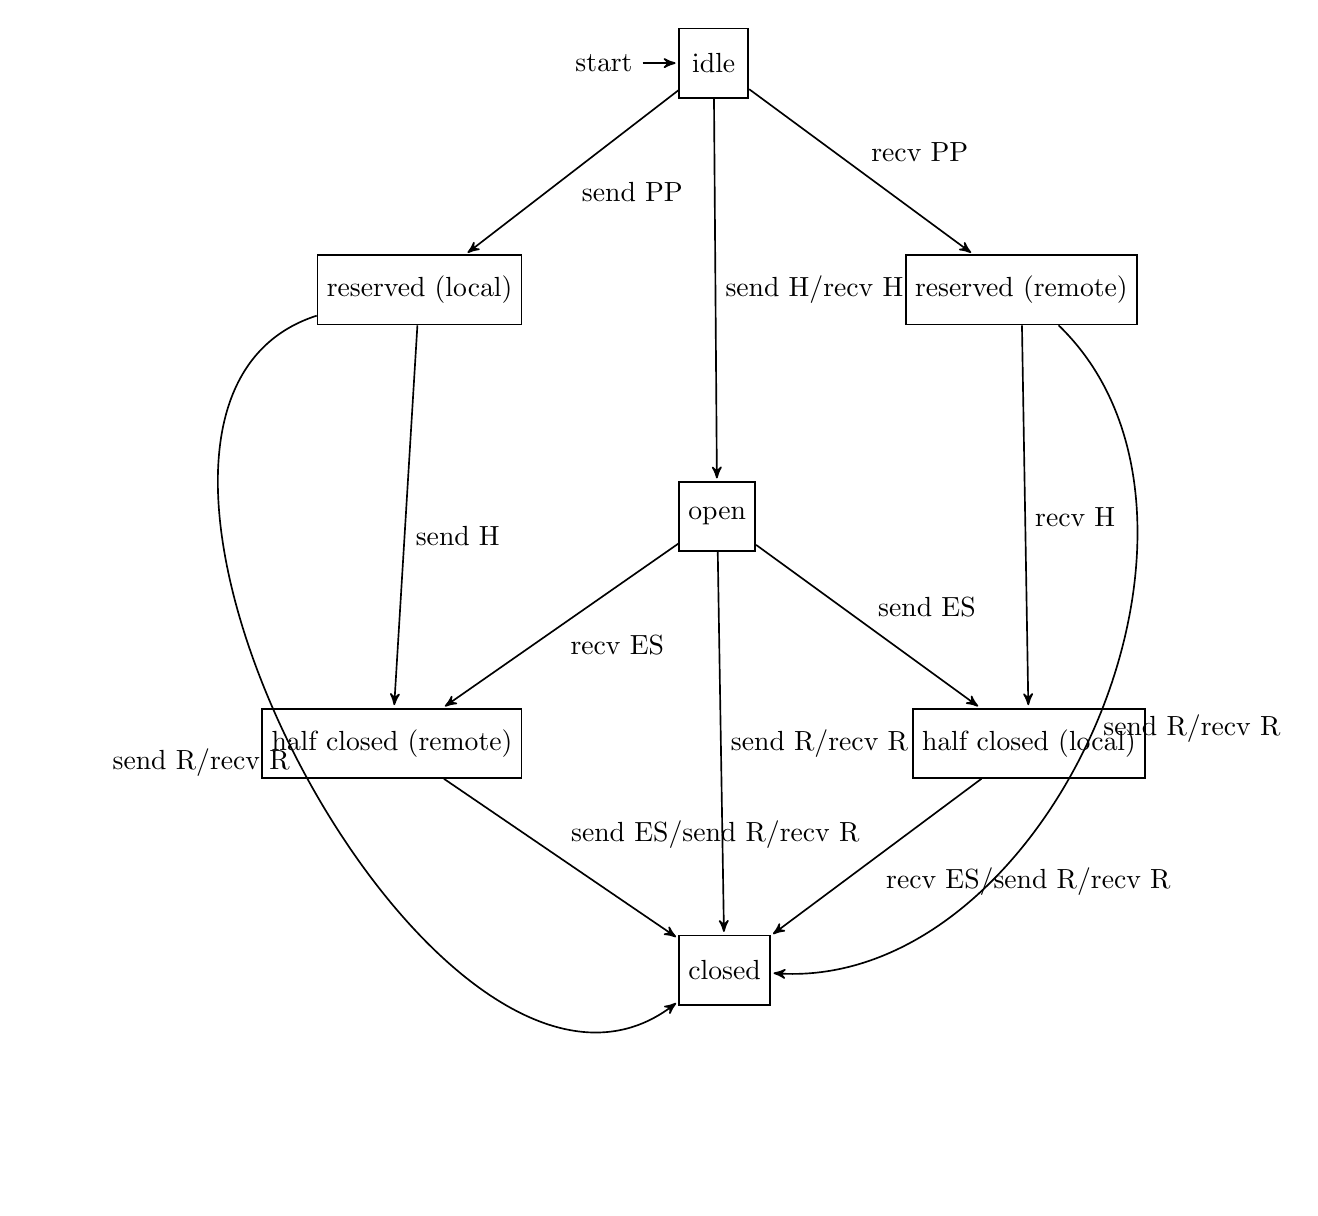
\begin{tikzpicture}[->,>=stealth',shorten >=1pt,auto,node distance=2.8cm,
	semithick]
	\tikzstyle{every state}=[draw, rectangle]

	\node[initial,state](idle){idle};

	\node[state, below left =of idle](rsv_loc){reserved (local)};
	\node[state, below right= of idle](rsv_rem){reserved (remote)};
	\node[state, below right =of rsv_loc](open){open};

	\node[state, below left=of open](hc_rem){half closed (remote)};
	\node[state, below right=of open](hc_loc){half closed (local)};

	\node[state, below right=of hc_rem](closed){closed};


	\path (idle) edge node {send PP} (rsv_loc)
	(idle) edge node {recv PP} (rsv_rem)
	(idle) edge node {send H/recv H} (open)
	(rsv_loc) edge [bend right=100] node[left] {send R/recv R} (closed)
	(rsv_rem) edge [bend left=70] node[right] {send R/recv R} (closed)
	(rsv_loc) edge node {send H} (hc_rem)
	(rsv_rem) edge node {recv H} (hc_loc)
	(open) edge node {recv ES} (hc_rem)
	(open) edge node {send R/recv R} (closed)
	(open) edge node {send ES} (hc_loc)
	(hc_rem) edge node {send ES/send R/recv R} (closed)
	(hc_loc) edge node {recv ES/send R/recv R} (closed)
	;

\end{tikzpicture}

http://http2.github.io/http2-spec/index.html\#StreamStates


\section{Performance of Web Traffic on Multipath TCP}


%HTTP/1.1 mostly benefits from Multipath TCP for larger file downloads because the TCP connections are often closed after one download, whereas the overhead of establishing auxilliary paths is not worthwile for downloading only one small file. In some studies it has been shown that the HTTP/1.1 performance is worse with MPTCP that with single path TCP on the same connection. Especially the common HTTP/1.1 optimization practice of sharding (spreading files among many different origins).
 
Inherent in Multipath TCP operation is some overhead of discovering and establishing multiple paths when the connection is set up. Older versions of HTTP use many short-lived TCP connections, so the overhead of multipath initialization can shatter the performance improvements of Multipath TCP. Combined with unmatched expectations of the browser, there are situations where Multipath TCP can hurt the HTTP/1.1 performance compared with single path TCP \cite{han2015mwebmptcp}.



\section{Measuring Web Performance}
\cite{han2015mwebmptcp}

%	1. PageLoadTime (Zeit bis Load Event)
%	2. Zeit bis DOMContentLoaded Event
%	3. First Paint / First Contentful Paint / First Meaningful Paint
%	> First Meaningful Paint is essentially the paint after which the biggest above-the-fold layout change has happened, and web fonts have loaded. See the spec to learn more: First Meaningful Paint: A Layout-Based Aproach.
%	https://developers.google.com/web/tools/lighthouse/audits/first-meaningful-paint
%	``Time to First Meaningful Paint: A layout-based approach''
%	https://docs.google.com/document/d/1BR94tJdZLsin5poeet0XoTW60M0SjvOJQttKT-JK8HI/view#heading=h.tdqghbi9ia5d

%1 und 2 sind �ber chrome remote debugging api leicht erh�ltlich (Page.loadEventFired)
%3 ist im Devtools Timeline view sichtbar, muss also auch �ber das remote debugging api verf�gbar sein (Devtools verwenden selber auch das rda)

%Chrome Debugging - Tracing
%https://chromedevtools.github.io/debugger-protocol-viewer/tot/Tracing/
%https://docs.google.com/document/d/1CvAClvFfyA5R-PhYUmn5OOQtYMH4h6I0nSsKchNAySU/edit



\subsection{Categorizing web page components}

%Automatische Einstufung von Seitenbestandteilen (HTTP Requests) in Relevanz / User Utility
%-> nicht Thema der Arbeit, aber evtl. relevant f�r praktische Umsetzung

%Automatisches Aufbauen von Dependency Graphs


\section{Cooperation of Application Layer and Transport Layer}

% technical problems to be solved:
% *api needs to be defined
% *there might be a layer in between (Presentation Layer, TLS omnipresent today)

There are two main technical challenges in cooperation between (network) layers:

The first is that an adequate API needs to be defined. This is tricky especially in our case, the cooperation of application and transport layer, as one side is in user space and the other is a kernel component in modern operating systems.

The second challenge results from the fact that these layers are not directly adjacent to each other: In our case it is TLS encryption, which operates in the presentation layer, making all application layer data opaque to layers below. Therefore, a side channel needs to be established to allow information flow around the TLS encryption.
% see also: security considerations...


% research: what kinds of information that one layer has available, could provide an advantage to an other layer

research: what kinds of information that one layer has available, could provide an advantage to an other layer

\cite{Raisinghani_2004}
\cite{nowlan2012unorderedtcp}




%=====================================================================
\chapter{Approach}
%=====================================================================


	
%Annahmen:
We will describe a few assumptions made for the implementation and all optimizations.
%TCP-Verbindung wird immer vom Browser aufgebaut
First, we always look at a MPTCP connection which is established by the web browser and accepted by the web server. This is always the case for HTTP connections.
%Nur der Client/Browser hat mehrere Interfaces / sendet MP JOIN Anfragen -> path-manager erstmal nicht relevant
Only the client has two interfaces with different network addresses. After the connection is set up, it directly opens the second subflow by connecting to the server from the secondary interface with a \code{MP_JOIN} option in the \code{SYN}. The server has only one (visible) interface and accepts the second subflow. Therefore we won't discuss different MPTCP path management algorithms.
%Client hat zwei Interfaces (Wi-Fi und 3G)
The client's interfaces are either Wi-Fi and 3G/LTE, as found on smart phones, or Ethernet and Wi-Fi, which is common for notebooks.
%Kontrollierbare Aspekte: 
%	- Scheduler
%	- TCP Flow Control/Congestion Control


\section{Metrics for Web Performance } \label{metrics-web-perf}



When evaluating the performance of web page loads, there are several metrics 
to look at. We use three timing metrics, which are available in the Google 
Chrome web browser's developer tools.

%Parameters/Properties/Values: (in order of usual occurence)
% ...stimmt nicht,domcontentloaded und firstmeaningfulpaint k�nnen in beliebiger abfolge auftreten, je nach dem wie die webseite angelegt/optimiert ist


% DOMContentLoaded
The \textit{DOMContentLoaded} event is fired after the main HTML document has 
been fully received and parsed by the browser \cite[section 12.2.6]{HtmlStandard}. 
As the parsing is blocked by synchronous JavaScript\footnote{Modern browsers 
use ``speculative parsing'', where parsing continues while waiting for the 
synchronous JavaScript to be loaded and run. Still, the browser can only fire 
\textit{DOMContentLoaded} after running all synchronous scripts, because 
scripts could confuse\footnotemark~ the parser and force it to parse the code 
after the \code{<script>} tag again.   
}\footnotetext{\url{https://developer.mozilla.org/en-US/docs/Web/HTML/Optimizing_your_pages_for_speculative_parsing}}, 
this event can't be fired before scripts have been downloaded and executed. 
Loading style sheets does not block parsing, but it is recommended\footnote{%
This recommendation is no longer valid for browsers which employ ``speculative 
loading'', a technique where resources referenced after script tags are 
downloaded in parallel.} to reference them before JavaScript files, so they 
will usually be loaded as well. 
%''The DOMContentLoaded event is fired when the initial HTML document has been completely loaded and parsed, without waiting for stylesheets, images, and subframes to finish loading.'' ~https://developer.mozilla.org/en/docs/Web/Events/DOMContentLoaded

%browsers can render before domcontentloaded, but are very relucant to do so. only if loading the document itself takes several seconds, they start rendering. they display a white screen or the web page that was open before 


% First Meaningful Paint
The \textit{First Contentful Paint} is the time when the first text, image or 
similar object is painted on screen. On most pages, the first object is a 
header or navigation bar \cite{Sakamoto2016TTFMP}, making this metric less 
useful for the purpose of measuring the time until useful content for the user 
is visible. We use the \textit{First Meaningful Paint} metric instead, which 
\textcite{Sakamoto2016TTFMP} defines as ``the time when page's primary content 
appeared on the screen.'' They emphasize that ``[d]efinitions of primary 
content differ depending on pages. For blog articles, it would be the headline 
+ above-the-fold text (and text must be visible -- not waiting for fonts). For 
search engines, it would be search results. If an image is critical to the page 
(e.g. e-commerce product page), then first meaningful paint requires it to be 
visible.'' Therefore, to measure the first meaningful paint accurately, it would 
be necessary for the user to define the primary content. In the developer tools 
of Google Chrome, it is implemented using a heuristic based on the number of 
layout objects, page height and web font loading.



% Page Load Time (i.e. time until the onLoad event)
The third metric we measure is the \textit{Page Load Time}, i.e. the time of 
the \textit{load} event. This is the time it takes to load all embedded 
resources, like style sheets, web fonts and images. 

A Python script is used to instrument the browser to load pages, and to record 
the times at which the events noted above occur over the Chrome Debugging 
Protocol. This is described in detail in Section \ref{measurement-script} in 
the implementation chapter.

In addition to timing metrics, we also look at the amount of bytes transferred, 
and the number of HTTP transactions made.
At the browser level, we measure the amount of bytes transferred and the number 
of transactions per request content type. This is further differentiated by 
whether the request finished before or after the DOMContentLoaded event, as a 
heuristic of whether the request was necessary for the initial rendering. We 
would have preferred the First Meaningful Paint here, but it is not available 
in real-time during the measurement.

We also measure the amount of bytes transmitted and received at the network 
level, so we can separately measure per subflow. This metric allows us to see 
how well the scheduling algorithm makes use of multiple subflows. On the other 
hand, if we have subflows with different cost, like metered mobile data, this 
allows us to evaluate how cost-effective our algorithm is.




\section{Analysis of Web Page Structure} \label{approach-web-analysis}


Modern web pages consist of dozens of resources. In this section, we analyze 
popular web pages with regards to the requests which are made by the browser 
to load them. Requests can be categorized by their type, so first, we go 
through the most common types of requests. 

\subsection{Request Content Types}

The \textit{Document} is the main HTML file which is loaded first. It is 
strictly necessary for the browser to render the page. It is also usually 
required for loading subsequent resources, because it contains their addresses. 
This requirement can be avoided by using the HTTP/2 push feature, but this has 
other drawbacks. Further \textit{Document} requests can be triggered by 
subframes in the top document.

\textit{Script} requests load either synchronous or asynchronous JavaScript 
resources. The synchronous ones, \code{<script>} tags without the \code{async} 
attribute are required by the browser to continue constructing the Document 
Object Model (DOM) tree. They are loaded as soon as the tag is parsed by the 
browser, and block the parsing and display of all content which is placed 
after them in the document.

\textit{Stylesheet}s are needed for the first layout cycle of the page, which 
means usually that nothing is displayed to the user until they are fully 
loaded. If they are loaded too slowly, the bare page without style sheets 
applied will be displayed, leaving a bad user experience. If the page uses web 
fonts, the text content of the page won't display until the corresponding 
\textit{Font} requests have finished.

\textit{Image}s can be loaded after the base frame of the site is visible, 
especially if the image size is provided in the Document source. The same is 
true for \textit{Media} like video and audio, as well as most \textit{XHR} 
requests. 

\subsection{}

To acquire a general overview of structure of requests on popular web sites, 
we took the 50 highest ranked sites
%\footnote{The number 50 results from the fact that only the first 50 sites 
%are available for free from the Alexa web site.}
 from the Alexa top sites lists\footnote{\url{http://www.alexa.com/topsites}} 
in the categories global, news and science. As only the home pages are listed, 
we added twelve news articles from top international and German news sites. 
We loaded these web pages in a web browser which we instrumented as described 
in Section \ref{metrics-web-perf}. 

%alexa_all - 50 top sites
%alexa_news - 50 top news sites (these are the homepages of the news sites)
%alexa_science 50 top sites form category 'science'
%news_article - 12 news articles from news sites listed in alexa_news and some german news sites


%note that we only measured requests before the onLoad event
%- usually web sites are finished with the onLoad event
%- e.g. google.com only starts loading its javascript after onLoad, but it is not necessary - site works without js
%- 
\begin{figure}
	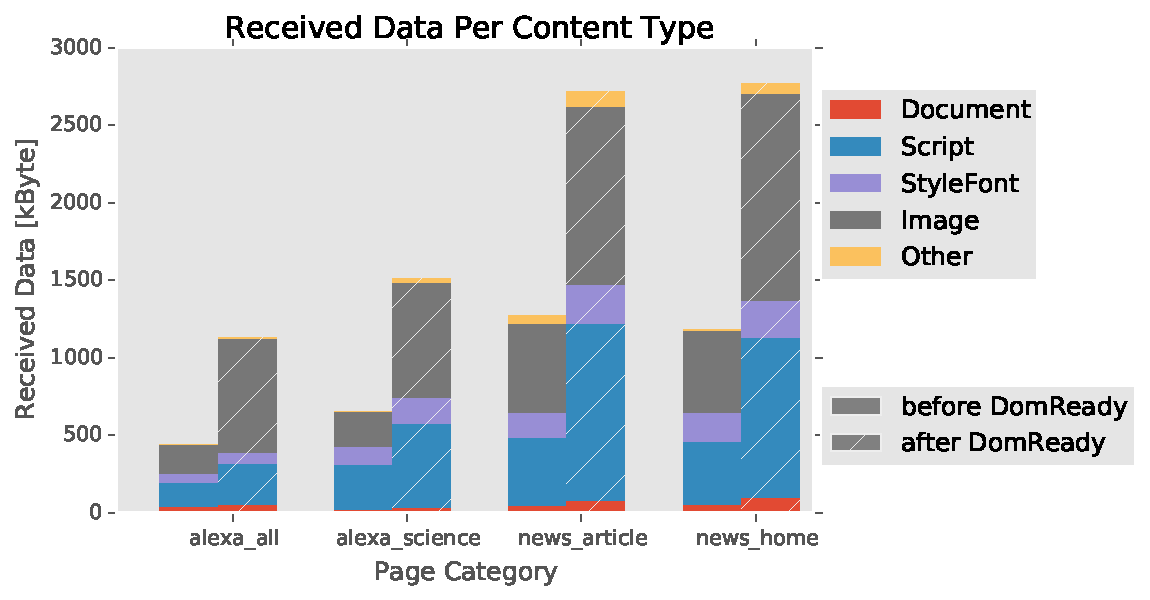
\includegraphics[width=0.9\textwidth]{wps-stackedSizeByCategory2.pdf}
	\caption{Transferred Data For Loading Web Pages, Grouped By Page Category, 
	Content Type And Relevance For DOM }
\end{figure}

\begin{figure}
	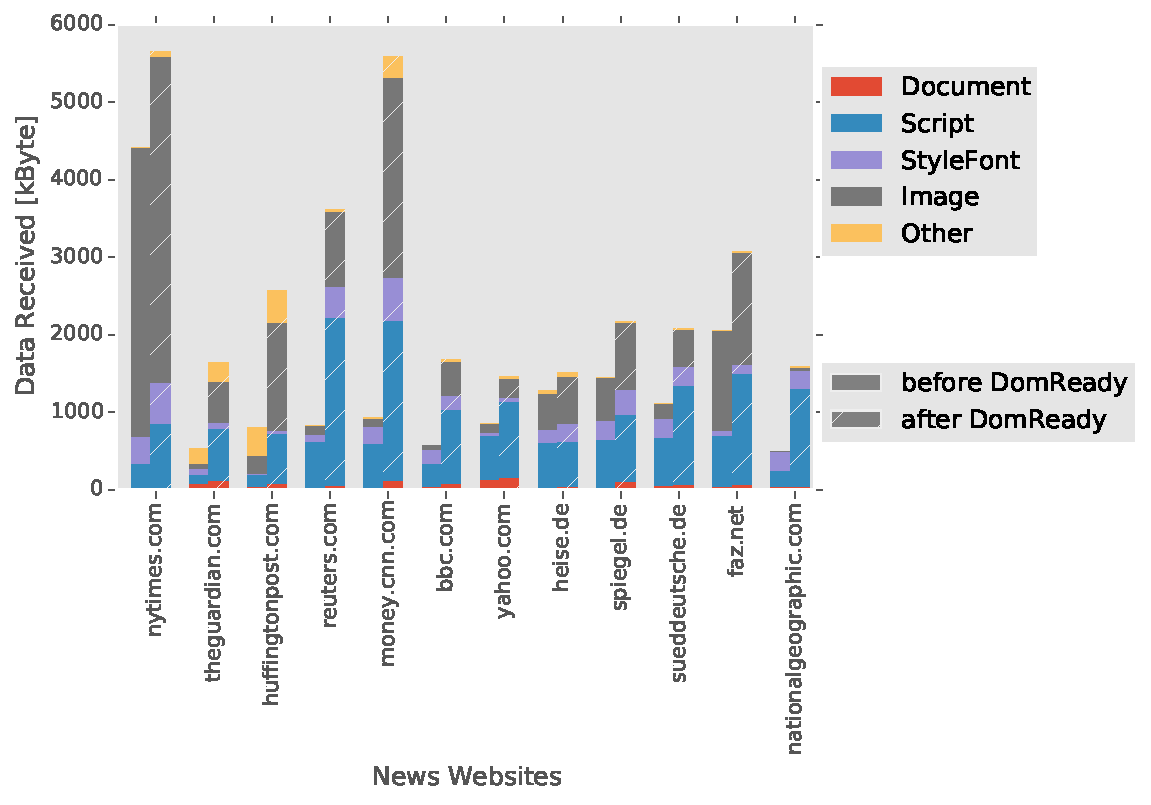
\includegraphics[width=0.9\textwidth]{wps-stackedSize-newsArticles.pdf}
	\caption{stackedSize-newsArticles}
\end{figure}


\begin{figure}
	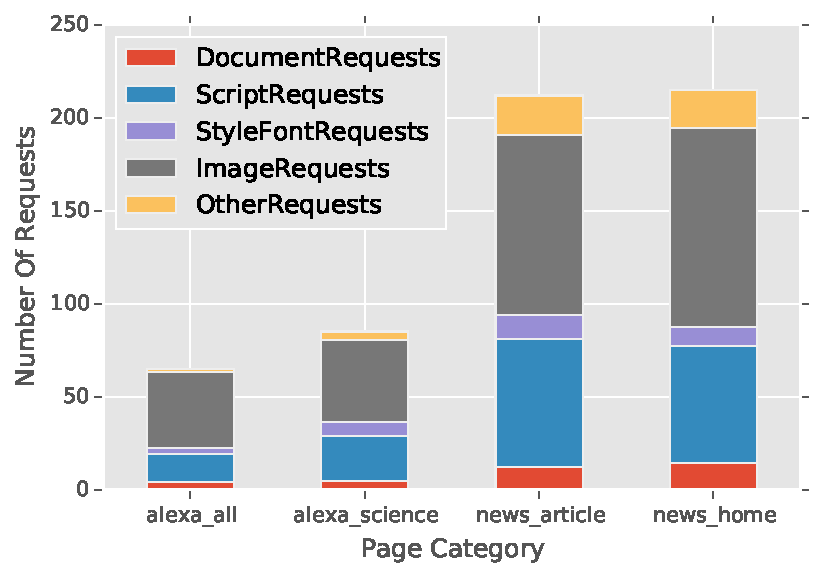
\includegraphics[width=0.9\textwidth]{wps-requestCountByCategory.pdf}
	\caption{requestCountByCategory}
\end{figure}

\begin{figure}
	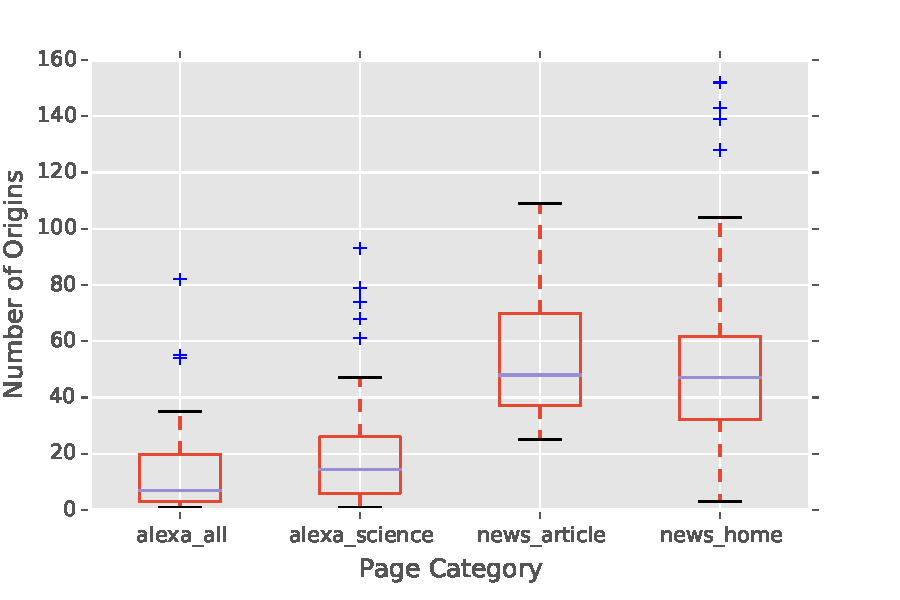
\includegraphics[width=0.9\textwidth]{wps-originCountByCategory.pdf}
	\caption{originCountByCategory}
\end{figure}




\section{Interaction between Transport and Application Layer} \label{approach-interaction}

%Wie dem Scheduler mitteilen was er tun soll?
%Problem: Wie erfolgt Kommunikation mit dem mptcp-scheduler? Zwischen mptcp und http2 sitzt in der regel noch tls! -> Paketinhalt f�r mptcp-scheduler nicht lesbar - evtl. �ber byte-counter


%Wo kommt die Logik hin?
%	- a: Server taggt Frames irgendwie, z.B. Inhalt=PageContent / Bild / Script / Style; Push=Ja/Nein; etc�, und Scheduler enth�lt die Logik die sagt was mit welchem Frame-Typ passieren soll
%oder b: Server gibt genaue Anweisung an Scheduler, dieser setzt es nur um
A decision we need to make is where to place the optimization logic. One approach is that the server tags every HTTP/2 frame with information like content or stream type, and the scheduler script decides that to do exactly. This way, there is maximum flexibility for the MPTCP configuration and the server doesn't need to know very much about MPTCP. On the other hand, we need special handling on the scheduler level for every application protocol we want to optimize.
The other approach is to have several general scheduler algorithms, each with different performance trade-offs, while allowing the application to decide which scheduler algorithm should be enabled. This reduces the dependencies on the scheduler level, but required more MPTCP specific decision making on the application level. 





\section{Optimizing the Multipath TCP scheduler}

We consider several optimization approaches based on our analysis of web page structure and the approach to pass hints about content and priority to the scheduler.


\subsection{Switching the Scheduler Based on Content Type or Priority}

Many modern web pages consist of dozens of resources. They can be classified by their technical priority for rendering the page. 

The \textit{Document} is the main HTML file which is loaded first. It is strictly necessary for the browser to render the page. It is also usually required for loading subsequent resources, because it contains their addresses. This requirement can be avoided by using the HTTP/2 push feature, but this has other drawbacks. 

Synchronous JavaScript resources (\code{<script>} tags) are required by the browser to construct the Document Object Model (DOM) tree. They must be loaded as soon as the tag is parsed by the browser.

Style sheets are needed for the first layout cycle of the page, which means usually that nothing is displayed to the user until they are fully loaded. If they are loaded too slowly, an the bare page without style sheets applied will be displayed, leaving a bad user experience.

Images can be loaded after the base frame of the site is visible, especially if the image size is provided in the Document source. The same is true for video, audio and most AJAX requests. 

We can also look at the subjective utility as perceived by the user.

In the case of text heavy pages, like on news sites, the Document and some images are most useful to the user as that contains the content of the page. In these cases, the JavaScript resources are often providing tracking and advertising. They are very important for the web site operator but not useful (even annoying) for the user. Especially tracking scripts can be delivered with lower priority as they are invisible and not time critical.

For single page web applications and other interactive pages all the relevant content is loaded by JavaScript. Therefore, JavaScript resources have a high user utility here.

Modern browsers and speed-optimized web pages make sure that the resources with the highest technical priority are requested first. The HTTP/2 server can also facilitate this by pushing out high-priority resources with HTTP Push.

We can therefore try to single out resources with low technical priority and low subjective utility. By giving this as a hint to the scheduler, these might be transmitted only on a cheaper but slower subflow. On the other hand, the higher prioritized contents could be transmitted redundantly in case of a lossy connection.

The resources with high technical priority, especially if required for the first layout cycle, will be handled by a scheduler with emphasis on low latency. %
%latency critical stuff -> redundant if lossy
In case of a lossy connection, this could be a scheduler transmitting packets redundantly on all subflows, thereby minimizing delays caused by packet loss.
%latency critical stuff -> send on backup if backup has lower rtt
%\todo{...or send on low-rtt despite IS\_BACKUP}
%-> combine by checking for loss+rtt

After these high priority resources are sent out, a more bandwidth conserving scheduler can be used. For example, if one subflow has a higher cost than the other, we could prevent lower priority resources from being sent over this expensive path.



\subsection{Aggressive Transmission of Last Segments}
The transmitting application signals the state of its outgoing buffers to the scheduler. An interesting condition occurs when the HTTP server has no more data to send, and only a few segments are left in the scheduler's queue. This means only these few segments are missing so that a complete web page can be rendered for the user. The scheduler can try to push out the missing segments more aggressively: By temporarily ignoring the available congestion window for the left over bytes, or by retransmitting on all available subflows.





\section{Security Considerations}
The information passed from the HTTP server to the MPTCP scheduler creates a side channel bypassing TLS encryption. It needs to be considered whether the passed data or the observable scheduler decisions based on this data could help an adversary. Some information are only protected by HTTP/2 and would be exposed on HTTP/1.1 connections anyway, like the length of individual resources. Others, like the content type, might be not available to the attacker otherwise.






%=====================================================================
\chapter{Implementation}
%==============================================================================

For this work, we implemented and modified several pieces of software. We 
extended a web server to pass internal information to the kernel by setting TCP 
socket options. Therefore, this chapter contains the reasoning behind our 
choice of the web server to modify, as well as a detailed description of the 
modifications made. Furthermore, we implemented a set of scripts to instrument 
a web browser to load web pages, collect information about the process and 
aggregate it together with information from the operating system's network layer. 
We also extended a framework for the evaluation of different Multipath TCP 
schedulers to run aforementioned client and server components. Finally, we 
implemented a Multipath TCP scheduler as RBS script which takes advantage of the 
hints given by the web server.


\section{Choosing a Web Server Platform}

Information about the contents of encrypted HTTP/2 application data is only 
available with cooperation of the web server is required. More precisely, we 
want to set socket options with hints for the scheduler, depending on 
information from higher levels. Multiple web servers have been evaluated and 
based on the criteria set out below, a suitable basis for the implementation 
has been selected.

To be considered, the server must support HTTP/2, and support it with at least 
one common browser as client. As we want to implement low-level modifications 
in the web server, the source code has to be available, and the license must 
permit modifications. This is a strictly necessary criterion, but luckily, most 
available web servers are permissively open source licensed under Apache, MIT 
or similar licenses. To make the work more relevant for practical use, a 
popular web server should be used. Therefore, we started our evaluation with 
Apache HTTP Server and NGINX, the two most popular open source HTTP servers. 
Apache HTTP Server internally uses the third-party library Nghttp2 for its 
HTTP/2 support, which contains the reference HTTP/2 server implementation 
Nghttpd, which we also evaluated and finally selected.


% NGINX (Plus)
% nginx has a open-source (community) and a ``enterprise'' version (NGINX Plus)
The \textbf{Nginx} web server is available as Open-Source Nginx and as the 
commercial, closed-source \textit{NGINX Plus}. Only the commercial edition 
has full HTTP/2 support, while the open-source ngx\_http\_v2\_module\footnote{%
\url{http://nginx.org/en/docs/http/ngx_http_v2_module.html}} lacks the 
``Server Push'' feature.
% only NGINX Plus has full HTTP/2 support, in the open source version e.g., no http2 push is supported


% Apache HTTP Server
% bucket brigades are too complicated...
The \textbf{Apache HTTP Server} fully supports HTTP/2 with its mod\_http2 
module. The module is based on Nghttp2, an HTTP/2 C library. We investigated 
the inner workings of Apache HTTP Server, following the byte stream from 
libnghttp2 to OpenSSL and finally the TCP socket. These internals are based on 
the Apache Portable Runtime\footnote{\url{https://apr.apache.org/}} (APR) and 
the concepts of Filters, Buckets, and Bucket Brigades.  To implement our 
extension, we would have to add additional metadata to every Bucket, making 
sure that it isn't lost in intermediate Filters. Another possibility is to add 
a new type of metadata buckets\footnote{%
\url{https://httpd.apache.org/docs/trunk/developer/output-filters.html}}, 
inserting them between data buckets every time the metadata (e.g. content type) 
changes.

% Nghttpd
Aside from the library, the Nghttp2 project also provides reference client, 
server and proxy implementations. Their server, \textbf{Nghttpd}, promised to 
be much less complex than Apache, while being still based on the same library. 
It has only one layer of buffering between the ``output'' of libnghttp2 and 
\code{SSL_write}, the ``input'' of OpenSSL, making it easy to pass along 
metadata. Also, the whole server consists of just over 3000 total lines of 
C++ code. This led us to use Nghttpd as the basis for our implementation.

 



\section{Modifications to the Web Server}

\begin{figure}[b]
	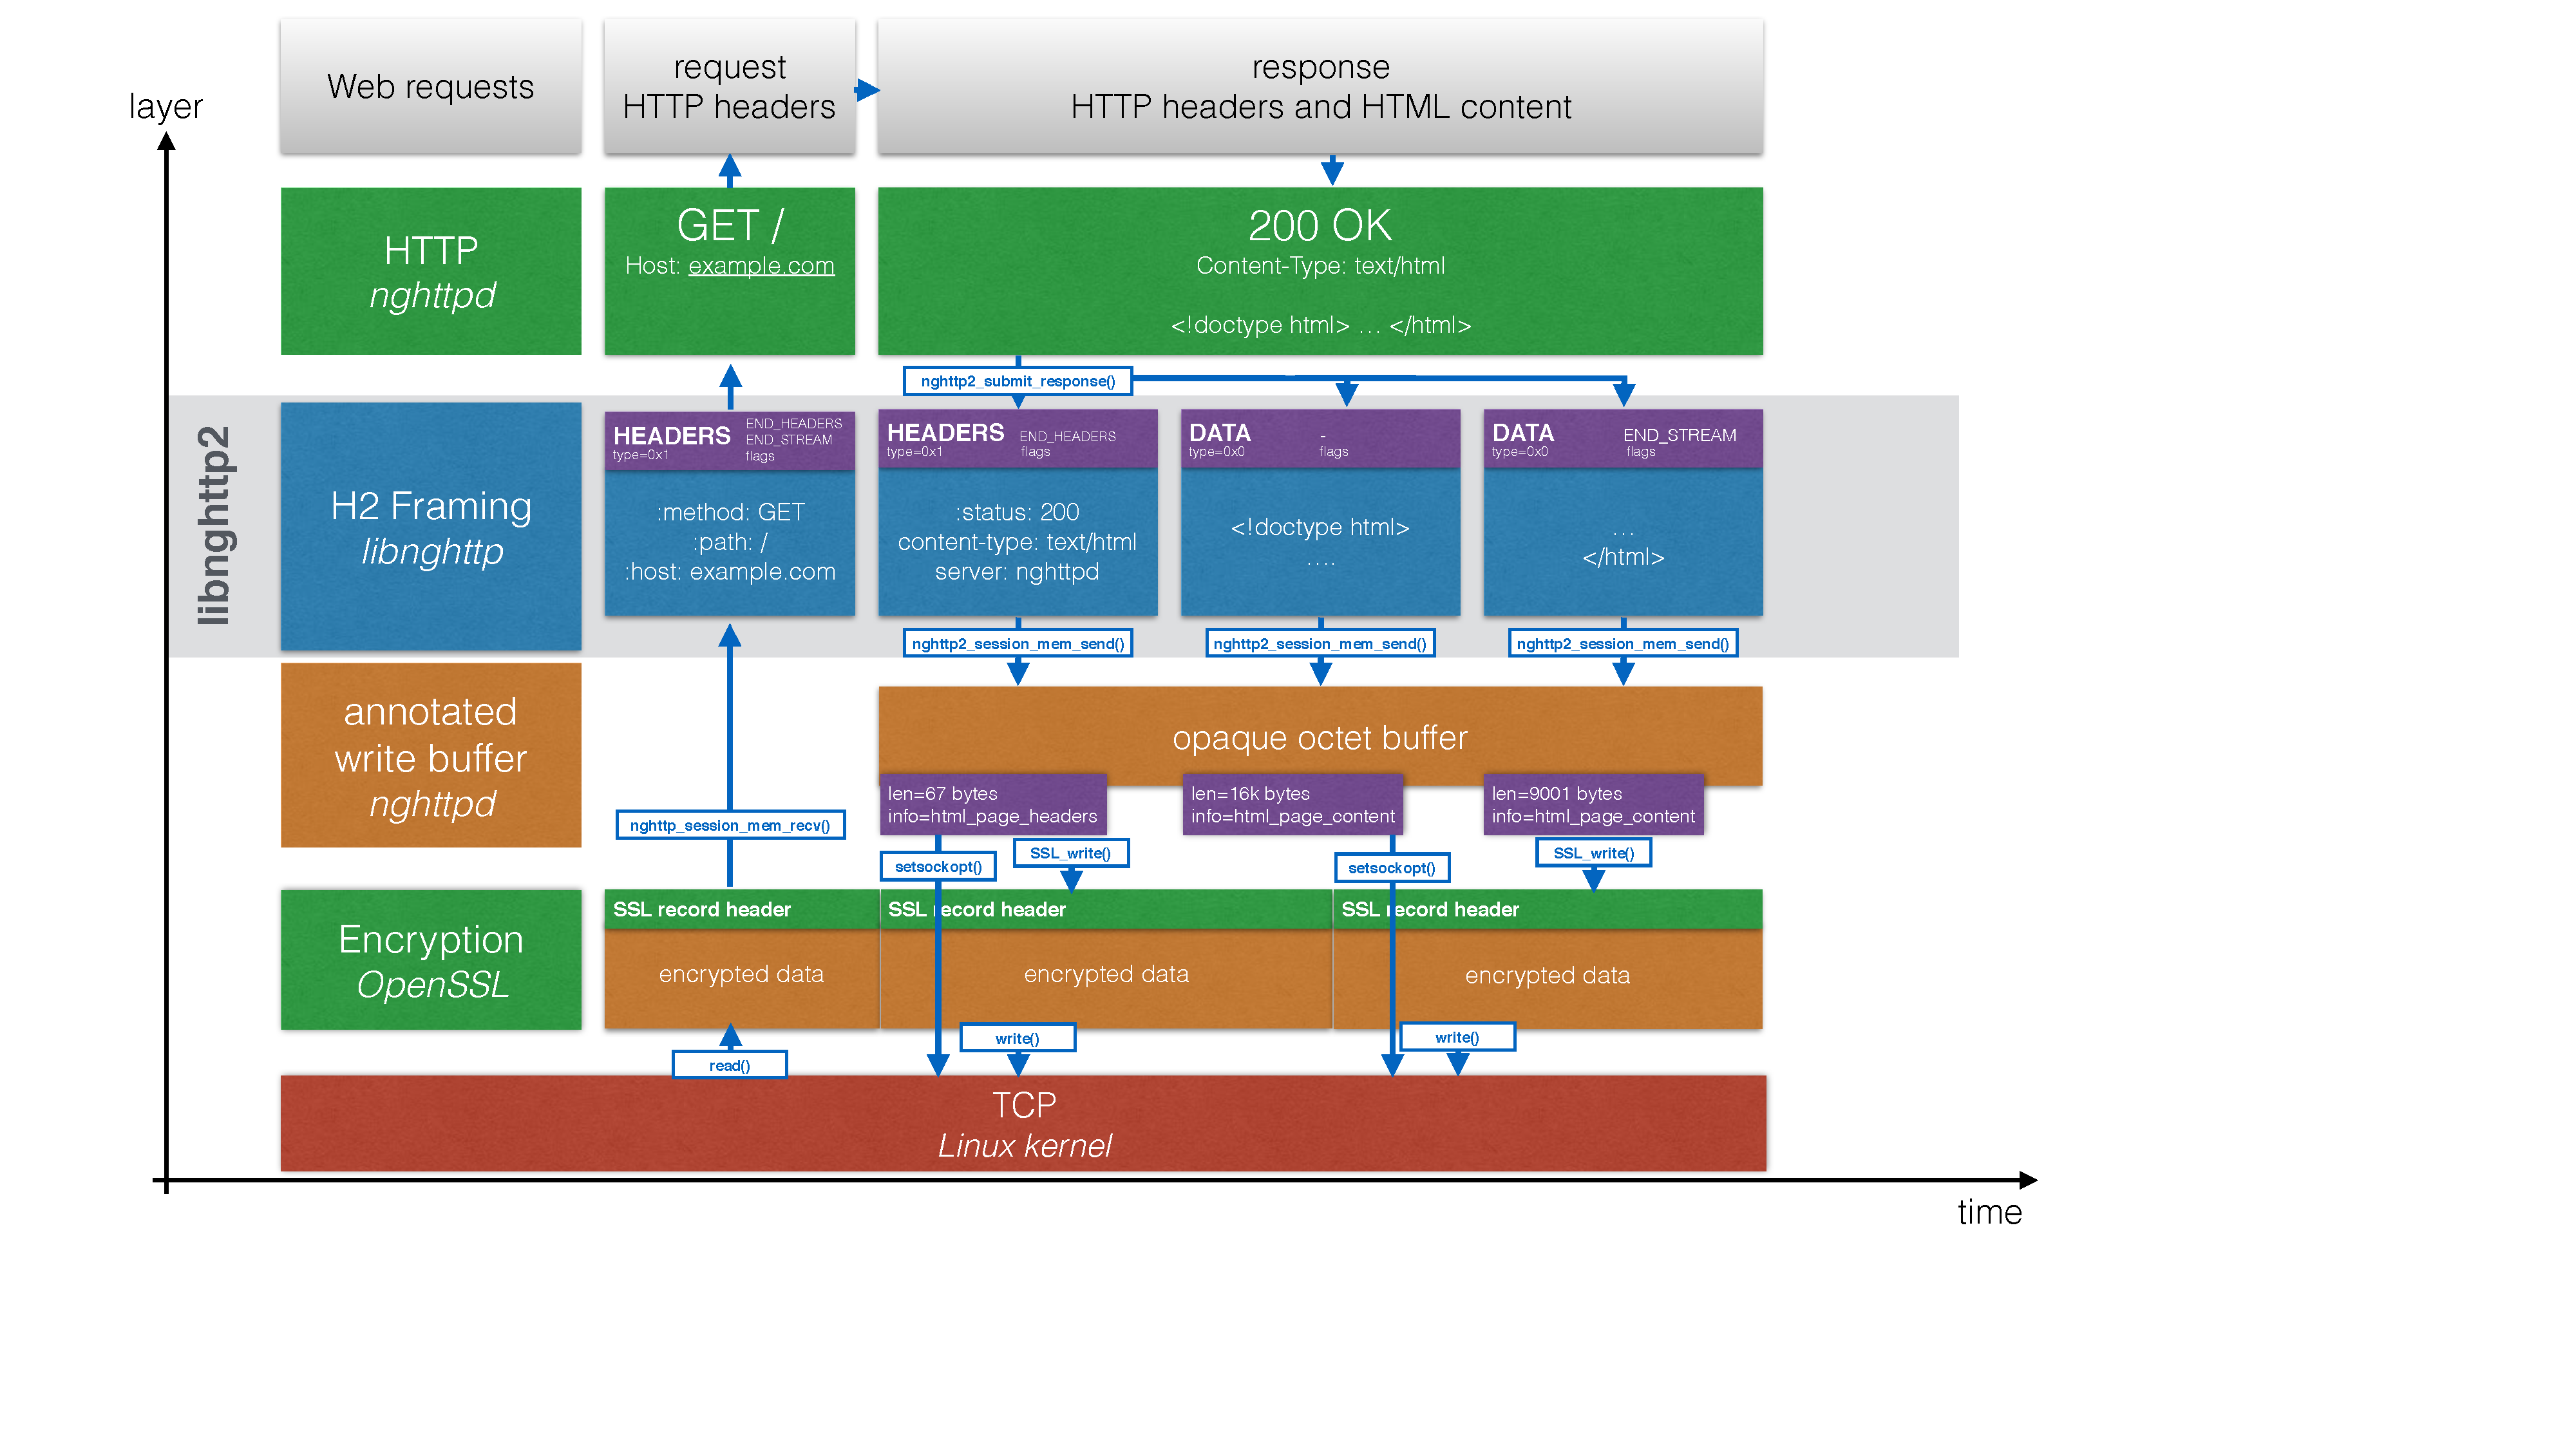
\includegraphics[width=1\textwidth]{http2-awb-layers.pdf}
	\caption{The annotated data's path through the application and network layer}
\end{figure}


\subsection{RBS Specific Modifications}
% selecting a RBS script for HTTP/2 connections (command line parameter)
\begin{lstlisting}[style=C_Code,label={lst:nghttpd_select_ruleset},caption={Extending Nghttpd's connection setup method to select a RBS script, excerpt of \code{HttpServer.cc}},numbers=left,firstnumber=281,linebackgroundcolor={\lstLinesAdded{284-295}}]
  void accept_connection(int fd) {
    util::make_socket_nodelay(fd);

#ifdef MPTCP_DEBUG
    printf("MPTCP: Selecting ruleset \"%s\" ...\n", config_->mptcp_ruleset.c_str());
#endif
    if (config_->mptcp_ruleset.length() != 0) {
      // configure MPTCP rule-based scheduler ruleset
      if (setsockopt(fd, IPPROTO_TCP, MPTCP_RULE_SET, config_->mptcp_ruleset.c_str(), 
			config_->mptcp_ruleset.length()) < 0) {
        perror("Error: Could not select ruleset for socket");
        close(fd);
        return;
      }
    }

    SSL *ssl = nullptr;
    if (ssl_ctx_) {
      ssl = ssl_session_new(fd);
      if (!ssl) {
        close(fd);
        return;
      }
    }
    auto handler =
        make_unique<Http2Handler>(this, fd, ssl, get_next_session_id());
    if (!ssl) {
      if (handler->connection_made() != 0) {
        return;
      }
    }
    add_handler(handler.release());
  }
\end{lstlisting}




% each HTTP/2 request is internally a Stream (in spec+server)
% store information about/in the stream: simplified content type -> priority
According to the HTTP/2 protocol specification, each transaction, or combination of request and response, is processed in a stream. Accordingly, Nghttpd has a \code{Stream} class which is instantiated for each request and stores relevant information. We extended this class by a \code{scheduling_content_type} field, which is a simplified representation of the transactions content type.


\begin{lstlisting}[style=C_Code,label=lst:mptcp_is_temp_unavailable,caption={Nghttpd's \code{struct Stream}, excerpt of \code{HttpServer.h}
%\footnote{url{https://github.com/multipath-tcp/mptcp/blob/e076f6be0f4b3d48d59c686d0a9ff4b87bc91a0f/net/mptcp/mptcp\_sched.c\#L39}}
},numbers=left,firstnumber=142,linebackgroundcolor={\lstLinesAdded{156}}]
struct Stream {
  BlockAllocator balloc;
  RequestHeader header;
  Http2Handler *handler;
  FileEntry *file_ent;
  ev_timer rtimer;
  ev_timer wtimer;
  int64_t body_length;
  int64_t body_offset;
  // Total amount of bytes (sum of name and value length) used in
  // headers.
  size_t header_buffer_size;
  int32_t stream_id;
  bool echo_upload;
  uint32_t priority_file_type;   // --> for mptcp scheduler
  Stream(Http2Handler *handler, int32_t stream_id);
  ~Stream();
};
\end{lstlisting}


\begin{lstlisting}[style=C_Code,numbers=left]
592  unsigned int get_skb_property(const Config *config, int caller, nghttp2_frame *frame, Stream *stream) {
  [...]
602    switch(config->mptcp_skb_property_mode) {
603      case RBS_PROP_FRAMETYPE:
604        if (!frame) return 0;
605         return frame->hd.type;
606      case RBS_PROP_CONTENTTYPE:
607        if (!stream) return SKB_CONTENT_NOSTREAM;
608        return stream->scheduling_content_type;
	[...]
614    }
615  }
\end{lstlisting}



% setting scheduling hints as RBS_USER socket option

% content type 




\subsection{TLS}

% newer openssl version (apls support)

% changing the maximum ssl record size

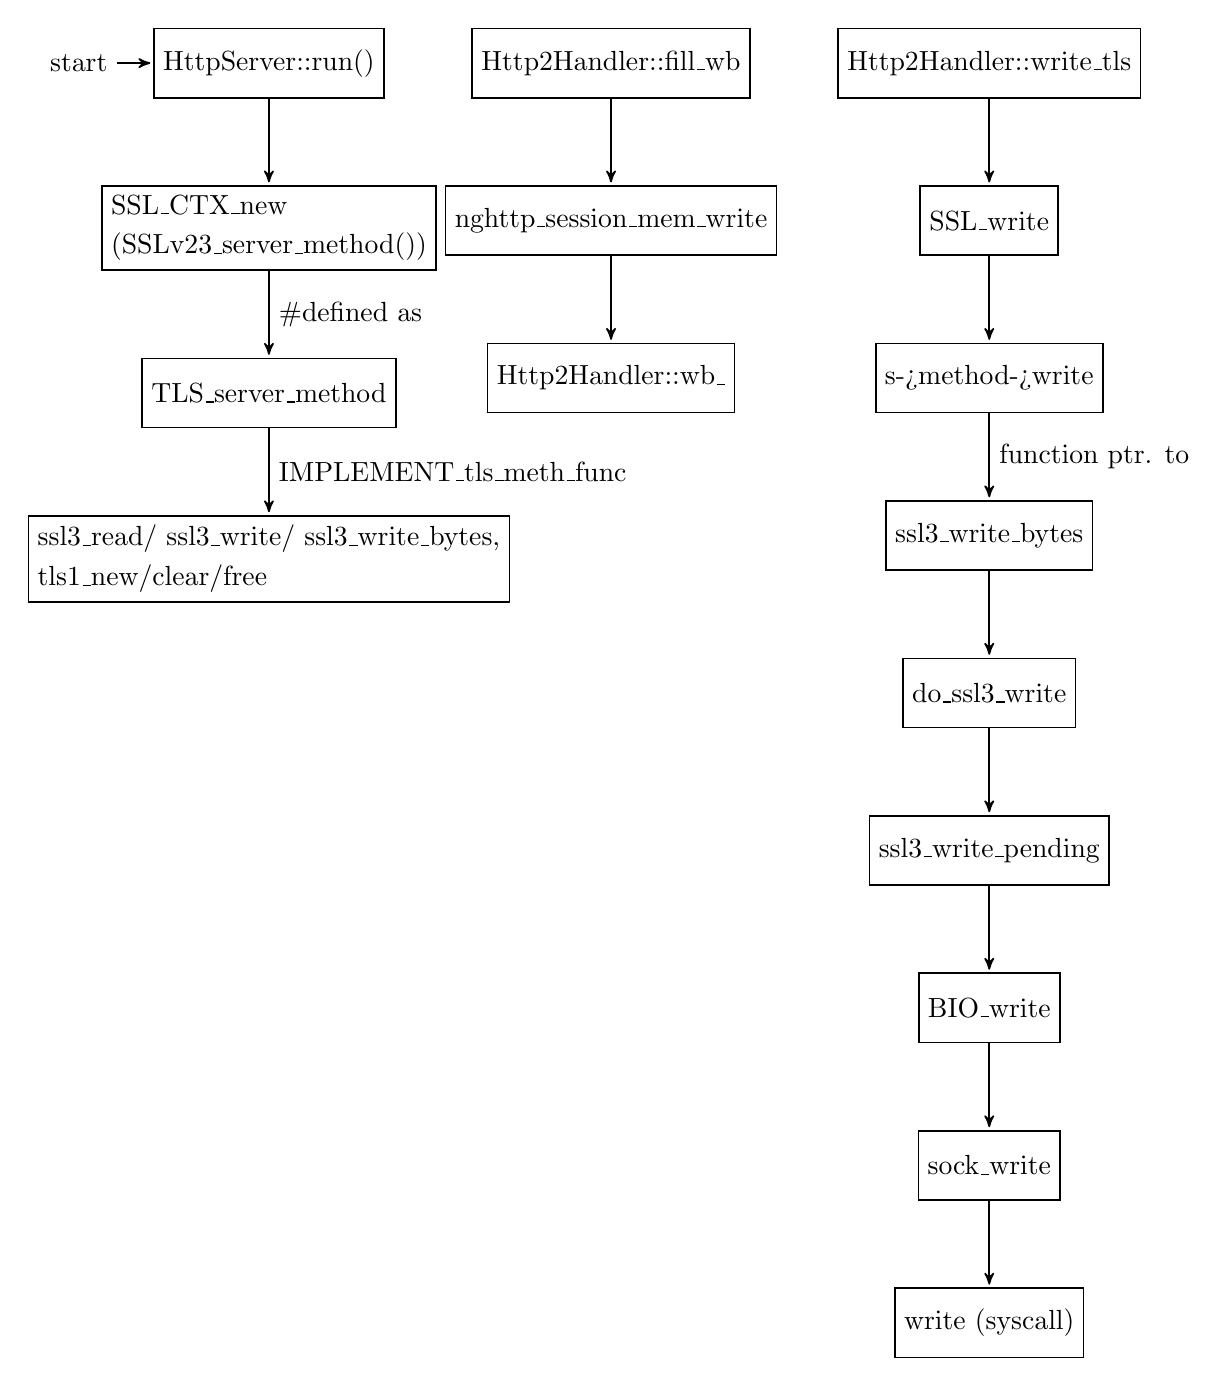
\begin{tikzpicture}[->,>=stealth',shorten >=1pt,auto,node distance=1.1cm,
		semithick]
	\tikzstyle{every state}=[draw, rectangle,
	execute at begin node={\begin{varwidth}{21em}},
	execute at end node={\end{varwidth}}]

	\node[initial,state](s1){HttpServer::run()};
	\node[state,below=of s1](s2){SSL\_CTX\_new \\(SSLv23\_server\_method())};
	\node[state,below=of s2](s3){ TLS\_server\_method  };
	\node[state,below=of s3](s4){ ssl3\_read/ ssl3\_write/ ssl3\_write\_bytes, tls1\_new/clear/free };


	\node[state,right=of s1](s6){  Http2Handler::fill\_wb };
	\node[state,below=of s6](s7){  nghttp\_session\_mem\_write };
	\node[state,below=of s7](s8){  Http2Handler::wb\_ };



	\node[state,right=of s6](s9){  Http2Handler::write\_tls };
	\node[state,below=of s9](sa){  SSL\_write };
	\node[state,below=of sa](sb){  s->method->write };
	\node[state,below=of sb](sc){  ssl3\_write\_bytes };
	\node[state,below=of sc](sd){  do\_ssl3\_write };
	\node[state,below=of sd](se){  ssl3\_write\_pending };
	\node[state,below=of se](sf){  BIO\_write };
	\node[state,below=of sf](sg){  sock\_write };
	\node[state,below=of sg](sh){  write (syscall) };

	\path (s1) edge (s2)
	(s2) edge node {\#defined as} (s3)
	(s3) edge node { IMPLEMENT\_ \\ tls\_meth\_func} (s4)

	(s6) edge (s7)
	(s7) edge (s8)

	(s9) edge (sa)
	(sa) edge (sb)
	(sb) edge node {function ptr. to} (sc)
	(sc) edge (sd)
	(sd) edge (se)
	(se) edge (sf)
	(sf) edge (sg)
	(sg) edge (sh)
	;


\end{tikzpicture}



\section{Schedulers}

%we use the <packet>.USER property and/or registers R1..6 set by the application code
%to choose the best possible scheduling preferences/modify the scheduling algorithm




%We use three timing metrics, which are available over the Chrome debugging protocol\footnote{\url{https://developer.chrome.com/devtools/docs/debugger-protocol}}, the protocol of the Google Chrome web browser's developer tools.

\section{Instrumenting the Web Browser} \label{measurement-script}

\begin{figure}
	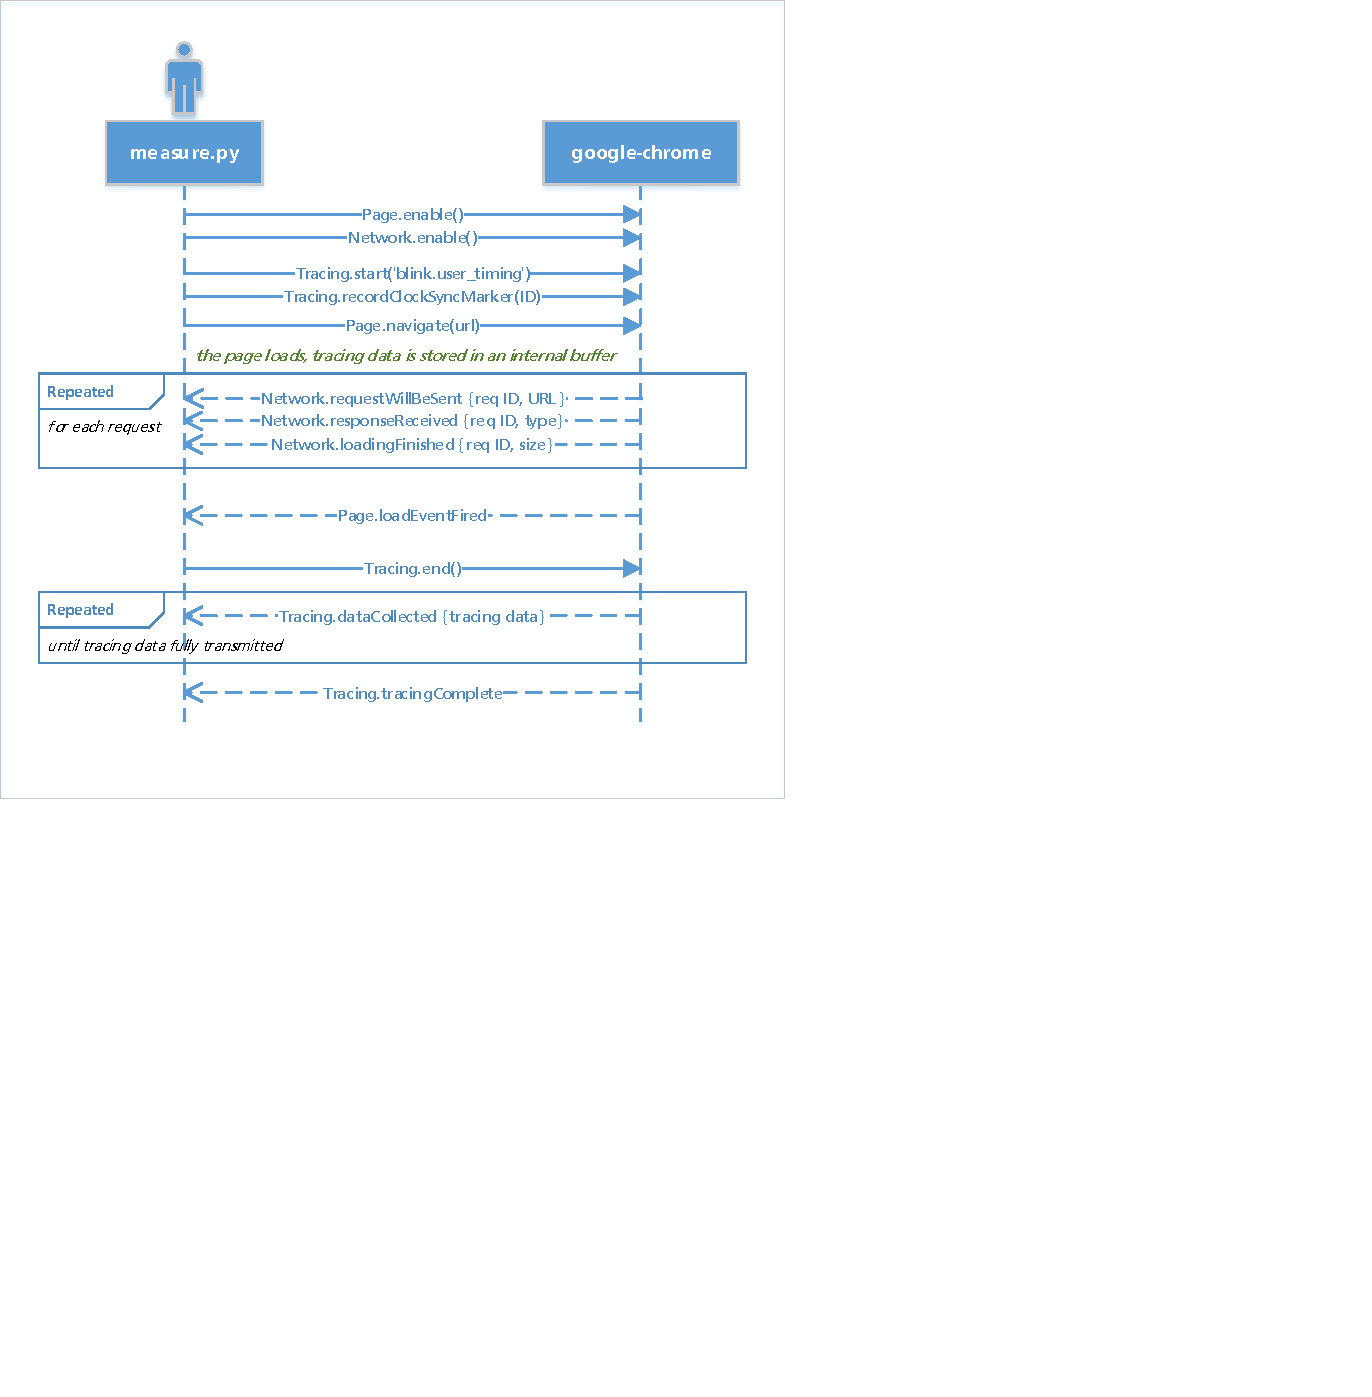
\includegraphics[width=0.8\textwidth, trim=0.25in 0.25in 0.25in 0.25in, clip]{chrome-tracing.pdf}
	\caption{A sample interaction with the Chrome Tracing API}
	\label{fig:chrome-tracing-api}
\end{figure}

In our analysis of web page structure, as well as in the later evaluations of 
collaborative schedulers, we use several metric as described in Section 
\ref{metrics-web-perf}. These are visible in the Google Chrome web browser's 
developer tools, and are available via the Chrome Debugging Protocol\footnote{%
\url{https://developer.chrome.com/devtools/docs/debugger-protocol}}. 
We use this protocol from a Python script, \code{measure_web_requests.py}, to 
instrument the web browser to navigate to pages we want to measure, and to 
retrieve the network and tracing data.

A sample interaction with the browser over the Chrome Debugging Protocol is 
shown in Figure \ref{fig:chrome-tracing-api}. The script first starts a new 
Chrome instance with special parameters to prevent interference: we disable 
automatic updates, the popup blocker, welcome message, Google Translate, and 
others. We also specify a new profile directory, to prevent distortion from 
cached data from previous experiments. 
After connecting over the Chrome Debugging Protocol, it enables \textit{Page} 
and \textit{Network} related events and starts a new tracing session. Because 
the tracing API uses its own timestamps, we need to synchronize it with wall 
clock time first by calling \textit{recordClockSyncMarker}. This allows us to 
combine tracing API timings with network API timings later.
The script will then ask the browser to navigate to the page we want to 
measure. While loading, the tracing component of Chrome stores all events in 
an internal buffer. The network component sends us events of every resource 
load in real time. We accumulate the number of requests and the response sizes, 
grouped by origin (domain name and port) and by content type.

As a result, the script prints a report as shown in Listing 
\ref{lst:measure-web-requests-output}. In this example, the English homepage of 
Wikipedia was loaded, which took 0.8 seconds in total. 310 kilobytes of data 
were transmitted from three different origins. 
In the second and third table, the column \texttt{\#req} shows the number of 
requests from this origin or of this DataType, respectively. 
The columns \code{xferAll} and \code{xferReady} give the kilobytes of data 
transmitted before the \textit{load} and before the \textit{DOMDocumentLoaded} 
event, respectively. The content types are listed in the third table. This 
allows us to see that document and stylesheets were fully loaded before the 
\textit{DOMDocumentLoaded} event, whereas most images loaded afterwards. 


\begin{lstlisting}[label=lst:measure-web-requests-output,caption={
	Excerpt from the output of \code{measure_web_requests.py}
},keywords={},numbers=left,tabsize=8]
(*\aftergroup\bfseries*)URL: https://en.wikipedia.org/wiki/Main_Page
Timings:(*\aftergroup\mdseries*)
0.0000  navigationStart
0.0002  fetchStart
0.0842  unloadEventStart
0.0842  unloadEventEnd
0.0845  domLoading
0.1113  responseEnd
0.2112  domInteractive
0.2112  domContentLoadedEventStart
0.2112  domContentLoadedEventEnd
0.3612  firstLayout
0.3708  firstPaint
0.3708  firstTextPaint
0.3708  firstContentfulPaint
0.3708  firstImagePaint
0.7463  domComplete
0.7464  loadEventStart
0.8080  loadEventEnd
(*\aftergroup\bfseries*)before DOMContentReady: 64k
before Load: 310k
#req 	xferAll     	xferReady	origin(*\aftergroup\mdseries*)
  16	   67.76k	    0.00k	upload.wikimedia.org
  10	  241.99k	   64.32k	en.wikipedia.org
   1	    1.06k	    0.00k	login.wikimedia.org
  11	    0.00k	    0.00k	data:
(*\aftergroup\bfseries*)#req	xferAll     	xferReady	DataType(*\aftergroup\mdseries*)
   2	   17.34k	   17.34k	Stylesheet
   1	   18.10k	   18.10k	Document
  30	   93.55k	    5.05k	Image
   5	  181.82k	   23.83k	Script
\end{lstlisting}





%=====================================================================
\chapter{Evaluation}
%=====================================================================

We start this chapter by a presentation of the evaluation setup and the reasoning behind the choices. This includes the software used, the data points collected, and the web sites to test the optimizations on.
Thereafter, the gathered data is presented and analyzed.


% overview of the chapter

% 1. decisions we made which have an impact on the evaluation:
%  -- using real web sites / hand-crafted sample web sites
%  -- if real web sites: which web sites to measure, how to prepare them for measurement
% - evaluation setup:
%  -- which browser to use for measurement
% - measured data points:
%  -- amount of data transmitted (overall, per interface/subflow)
%  -- complete page load time (onLoad)
%  -- load time of HTML Document
%  -- time to DOM Ready (doc + blocking scripts)
%  -- time to first render/paint
%  -- time to ``above the fold ready'' (this is probably the closest to user impression of load time)
%     - can be measured as the time of the last change above the fold
%  -- time to ``text ready'' (useful e.g. on newspaper sites where most users want to read the content only/first, but lot of slow crap is shown above the fold)

% 2. how the measurement is conducted (used browser, used additional scripts/extension to gather data from browser, additional scripts to gather transmitted data from network stack client/server side, automation, ...)
% -> this could as well go into Implementation???

% 3. results: data, graphs, observations, conclusions...









\section{Selection of Sample Web Pages}

We have to decide which web sites to measure.

- Synthetic content / Self built test pages (plain html, small html file with many scripts/css, big html, etc ...)


Measuring the page load times of real-world web pages (mirrored on special web server under our control. Mirroring is necessary for multiple reasons: First, to ensure repeatability of the results we don't want the load of the ``real'' web server and the network connection in between to compromise our measurement. Second, we need the web server to support HTTP/2, which is not too common, and MPTCP, which is extremely rare in the wild)

- Alexa Top Sites (or similar ranking)

- Hand-selected sites with interesting features / problems / optimization potentials

- Sites which are often used on mobile



\section{Preparation of Real-World Web Pages}

% some can be used as is
Some real-world web pages can be used as is for evaluation by using the ``Save as'' option of a web browser. This is especially true for web sites with no content loaded with JavaScript and no third-party content.
% most web sites need to be prepared
Most web sites need to be prepared in one or another way. 
% on some, changes are inevitable, they won't work otherwise (https neccessary for h2, problems with third-party requests and dynamic content, etc)
Changes are inevitable when sites won't work otherwise. This is the case if the site is usually loaded over unencrypted HTTP, as for HTTP/2, browser enforce the use of TLS encryption. For third-party content, various possible solutions are discussed below.
% on some, we should change stuff, e.g. because there are optimizations for http/1.1 which make things worse on http/2 and it would be unrealistic to use them in this state
There are sites which we can test unmodified, but where we should change things to get more realistic results. For example, many sites use special optimizations which are tailored to HTTP/1.1, which make things worse on HTTP/2. One example of such optimizations is sharding\footnote{\url{https://www.nginx.com/blog/7-tips-for-faster-http2-performance/\#tip7sharding}}, a technique where resources on a page are spread over several domains, to overcome the limitation that web browser are only allowed to open a certain number of parallel connections to one domain. With HTTP/2, this slows down the page load because of the overhead of establishing many TCP and TLS connections, which are unnecessary as parallel downloads are now possible over a single connection.

% etc.



\subsection{Handling Dynamic and Third Party Requests}

As we found in Section \ref{approach-web-analysis}, most modern web sites request resources from third-party hosts, and refer to resources which are generated dynamically by the server, possibly changing with every request.
We have to handle these cases in our evaluation. 

%Downloading web pages with browser/wget and delivering with nghttpd - Problem: how to handle dynamic or third-party requests?


In these simulations, we chose to keep most third party requests as-is, loading the resource from the original server, especially advertisements, tracking snippets and complex libraries from Content Delivery Networks (CDNs). This has the advantage of providing more realistic results than rejecting all third-party requests at the browser or firewall level. 
Another possible approach would have been to implement an explicit or transparent HTTP/2 proxy, which caches all requests for a page load, and replays them for later evaluations. This has been implemented for HTTP/1.1 by the Chromium team in web-page-replay\footnote{\url{https://github.com/chromium/web-page-replay}}. 
Simple JavaScript libraries (consisting of single files) were downloaded and served locally, and we modifying the web page to fetch them from the local server. This is a simple optimization which is realistic to be made by real website operators.

% Cancel/reject all third party requests (in-browser / iptables)
%	Pro: Easy, reproducible
%	Con: not realistic (always a lot faster than real request)
%	Pro: might be faster by the same amount, so still comparable (?)

% Let all third party requests through to the original sites
%	Pro: Easy, realistic
%	Con: dependent on network condition of test computer and load on original server (not reproducible)

% Alternative: Use a caching HTTP/2 proxy (nghttpx, apache)
%	Pro: realistic (?), reproducible, (not that difficult either)
%	Con: ...



\section{Measurement Environments}

We based our measurements on two different methods. We simulated network situations with Mininet, which constructs a completely virtual environment on a single computer. This approach has the benefit of being fairly reproducible, because no-one else uses the virtual network and causes uncontrollable variations. On the other hand, the simulation only represents part of the reality, therefore we also conducted evaluations on real networks. This trades reproducibility for a more realistic environment, including congestion on intermediate routers, packet loss on Wi-Fi and cellular links, and other behaviour of real networks, which is quite complex.


\subsection{Mininet}

\todo{short intro to mininet}

\todo{our setup with mininet}

\todo{...}



\subsubsection{TCP Small Queues}

If there is a stall below the TCP layer, the TCP small queues \cite{LwnTSQ} algorithm ensures not too much data gets buffered in the fifos of network interfaces, e.g. when an applications send data faster than the network interface card can relay it. To do this, the algorithm checks \code{sk_wmem_alloc}, a field of the socket struct in the kernel, which stores the amount of memory currently used for the send buffer. The default multipath scheduler in the Linux kernel declares a subflow as temporarily unavailable if the underlying TCP socket is throttled, as seen in Listing \ref{lst:mptcp_is_temp_unavailable}. When using RBS, the information if a subflow is throttled is available as the property \code{<subflow>.THROTTLED} and can be considered in the scheduling decision.

\begin{lstlisting}[style=C_Code,label=lst:mptcp_is_temp_unavailable,caption={Excerpt from Multipath TCP Kernel, \code{net/mptcp/mptcp_sched.c}
%\footnote{url{https://github.com/multipath-tcp/mptcp/blob/e076f6be0f4b3d48d59c686d0a9ff4b87bc91a0f/net/mptcp/mptcp\_sched.c\#L39}}
}]
static bool mptcp_is_temp_unavailable(struct sock *sk,
				      const struct sk_buff *skb,
				      bool zero_wnd_test)
{
 [...]
	/* If TSQ is already throttling us, do not send on this subflow. When
	 * TSQ gets cleared the subflow becomes eligible again.
	 */
	if (test_bit(TSQ_THROTTLED, &tp->tsq_flags))
		return true;
\end{lstlisting}

This is where a difference between simulated and real networks exists: in Mininet the TCP Small Queue throttling never got engaged, because \code{sk_wmem_alloc} never changes from its initial value of \code{1}. This is consequential, as the virtual ethernet devices don't have to really transmit any data, instead only passing along a pointer, and therefore never need to buffer it.

In our simulations, each packet is delayed in the network emulation (netem) layer, and traffic shaping is used, to simulate a real link with latency and limited bandwidth. This layer resides between the TCP stack and the virtual ethernet device, therefore it should cause \code{sk_wmem_alloc} to increase, but it didn't.
%-        Gilt das auch f�r shaping ohne delay, e.g., 10 Mbit bw? W�rde es ohne den patch also mit 10Mbit und ohne delay �wie erwartet� laufen?
When using only traffic shaping, but not the delaying functionality of netem, the problem does not occur. 

%https://kernelnewbies.org/Linux_3.6#head-b1e33c4c78affb4186e5affc4b4a2bc7d44a3e66
%https://lwn.net/Articles/507065/

So we built a test case where a delay is added on one host with netem\footnote{\code{tc qdisc add dev h1-eth0 root netem delay 5000ms}}, and then \code{iperf} is run to create traffic between the host. We also added a debug output to the function \code{tcp_small_queue_check} in \code{net/ipv4/tcp_output.c} \footnote{\url{http://lxr.free-electrons.com/source/net/ipv4/tcp_output.c\#L2074}} to see if TSQ will throttle the output. But in Mininet / veth, \code{sk_wmem_alloc} is always at the value \code{1}. The \code{TSQ_THROTTLED} never gets set. If doing the same on two machines connected over ethernet cable, \code{sk_wmem_alloc} raises, and eventually \code{TSQ_THROTTLED} is set.

An inquiry on the Mininet mailing list resulted\footnote{\url{https://mailman.stanford.edu/pipermail/mininet-discuss/2017-April/007425.html}} in the hint that the latency emulation code calls \code{skb_orphan_partial}, which reduces the socket buffer's size to \code{1}, therefore essentially removing it from \code{sk_wmem_alloc}.
This further lead us to a code comment in the Linux kernel which says that this behaviour is by design, because ``orphaning usually takes place at TX completion time, so \_before\_ the link transit delay'' (Linux kernel 4.4, \code{net/sched/sch_netem.c}, line 429). 
%-        Netem delay packets werden EXTRA rausgenommen, weil?
The reason is that the netem layer is designed to emulate delays in the \textit{network}, not \textit{network interface}, to test e.g. TCP congestion control algorithms. Therefore it needs to behave as if the delay occured after orphaning the socket buffer.  But we want do emulate delays in the \textit{network interface} in this case, so we change this behaviour by commenting out the call to \code{skb_orphan_partial} as shown in Listing \ref{lst:sch_netem}. To see if the call would have been normally made, we also added a debug output temporarily. This enabled us to test the TSQ throttling in our simulation with Mininet.


\begin{lstlisting}[style=RBS,label=lst:sch_netem,caption={Modified version of Linux kernel 4.4, \code{net/sched/sch_netem.c}, line 398ff},linebackgroundcolor={\lstLinesRemoved{13-14}\lstLinesAdded{16-18}}]
/*
 * Insert one skb into qdisc.
 * Note: parent depends on return value to account for queue length.
 *      NET_XMIT_DROP: queue length didn't change.
 *      NET_XMIT_SUCCESS: one skb was queued.
 */
static int netem_enqueue(struct sk_buff *skb, struct Qdisc *sch)
{
 [...]
        /* If a delay is expected, orphan the skb. (orphaning usually takes
         * place at TX completion time, so _before_ the link transit delay)
         */
        // if (q->latency || q->jitter)
        //         skb_orphan_partial(skb);

        printk("netem_enqueue: ...not calling skb_orphan_partial, "
               "latency=%ld, jitter=%ld, sk=%p, sk_wmem_alloc=%d", q->latency, q->jitter,
               skb->sk, skb->sk == NULL ? 0 : atomic_read(&skb->sk->sk_wmem_alloc));
\end{lstlisting}








\subsection{Real World Measurements}

To confirm the measurements we conducted in Mininet, we ran the same software on real hardware and real networks. For the server side, we used a virtual machine located in the Frankfurt data center of Amazon Web Services and another one in the Roubaix data center of OVH. As clients, we used notebooks connected to the internet via Wi-Fi and DSL, via a Wi-Fi hotspot with VPN tunneling, and via USB to a mobile phone with an LTE connection.\footnote{We were unable to use the university's internet connection directly as its Firewall blocks Multipath TCP connections.}

\todo{more details about the measurement setup?}



\section{Evaluations}

\todo{something}

\subsection{Evaluation A (``Bad Wi-Fi'')}
% zeigen - implementiertung funktioniert grunds�tzlich
% simple (``academic'') content-type specific scheduling

The goal of this evaluation is to test the implementation of content-type specific scheduling, and to show a first content-type based optimization of a synthetic web page. The network situation is shown in Figure \ref{eva1-scenario}. A user with a smart phone is connected to a free Wi-Fi hotspot, which routes the traffic through a VPN and therefore incurs a high latency, and is also connected to a cellular network with low latency but metered traffic limits. The user loads a web page which is modelled after a typical news article, it consists of an HTML document referencing style sheet, script and images of different size. All styles and scripts are included in the \code{<head>} of the document and required for rendering the page. Two big images are included below the fold and are not required for the rendering.

The scenario is emulated in Mininet. Client and Server are modelled as Mininet hosts running the Google Chrome browser and the nghttpd web server, respectively. They each have two interfaces, which are connected by two Mininet links with delay and rate limiting to simulate the two connection paths. 

A scheduler script was designed to send the images only over the ``cheap'' Wi-Fi subflow, and allow the other, more time-critical data, to choose from the available subflows the one with the lowest round-trip time.


%story:
% situation: unmetered wifi hotspot with high latency, metered cellular with low latency
% results:
%  without mptcp - using only slow wifi - firstMeaningfulPaint X sec, load X sec
%  without mptcp - using only cellular - fast, but expensive
%  with 'stupid' mptcp - min_rtt scheduler, using both paths - firstMeaningfulPaint X sec, load X sec, uses lots of cellular data volume
%		-> because cellular has lower rtt, equal to cell only -> fast, but expensive
%  with 'intelligent' mptcp - min_rtt scheduler, using cellular only for 'important' stuff - firstMeaningfulPaint X sec, load X sec,
%			uses not that much cellular data, firstMeaningfulPaint as fast as cell only, but load slower -> compromise ``cheap and (kinda) fast''




%sudo python2 execute.py --congestion_control cubic --network badWifiHotspot -a http2 --scheduler 'min_rtt_ctype_aware.txt min_rtt_advanced.txt'
%badwifi.ipynb

\begin{lstlisting}[style=RBS,label=lst:sched_eval_a,caption={RBS Scheduler Script for Evaluation A (``Bad Wi-Fi'')},numbers=left]
/*
 * This scheduler sends packets on the subflow with the lowest RTT which has congestion window available
 *  ... except images, they are sent only on the "cheap" (non-backup) subflow (e.g. Wi-Fi instead of 3G)
*/
SCHEDULER min_rtt_ctype_aware;

VAR SKB_CONTENT_NOSTREAM = 1;
VAR SKB_CONTENT_DOCUMENT = 2;
VAR SKB_CONTENT_SCRIPT   = 3;
VAR SKB_CONTENT_STYLE    = 4;
VAR SKB_CONTENT_IMAGE    = 5;
VAR SKB_CONTENT_OTHER    = 6;

/* only use subflows which have CWND left*/
VAR usableSbfs = SUBFLOWS.FILTER(sbf => sbf.CWND > sbf.SKBS_IN_FLIGHT);

/* no subflows available? do nothing. */
IF (usableSbfs.EMPTY) { RETURN; }

/* send packets from resend buffer redundantly on the fastest new subflows */
IF (!RQ.EMPTY) {
	usableSbfs.FILTER(sbf => !RQ.TOP.SENT_ON(sbf)).MIN(sbf => sbf.RTT).PUSH(RQ.POP());
	RETURN;
}

IF (!Q.EMPTY) {
	/* simplified content type is passed along by the web server */
	VAR content_type = Q.TOP.USER;

	IF (Q.TOP.USER >= SKB_CONTENT_IMAGE) {
		/* the subflows marked as "BACKUP" are filtered out */
		usableSbfs.FILTER(sbf => !sbf.IS_BACKUP).MIN(sbf => sbf.RTT).PUSH(Q.POP());
	} ELSE {
		usableSbfs.MIN(sbf => sbf.RTT).PUSH(Q.POP());
	}
}
\end{lstlisting}


\begin{figure}
\centering
	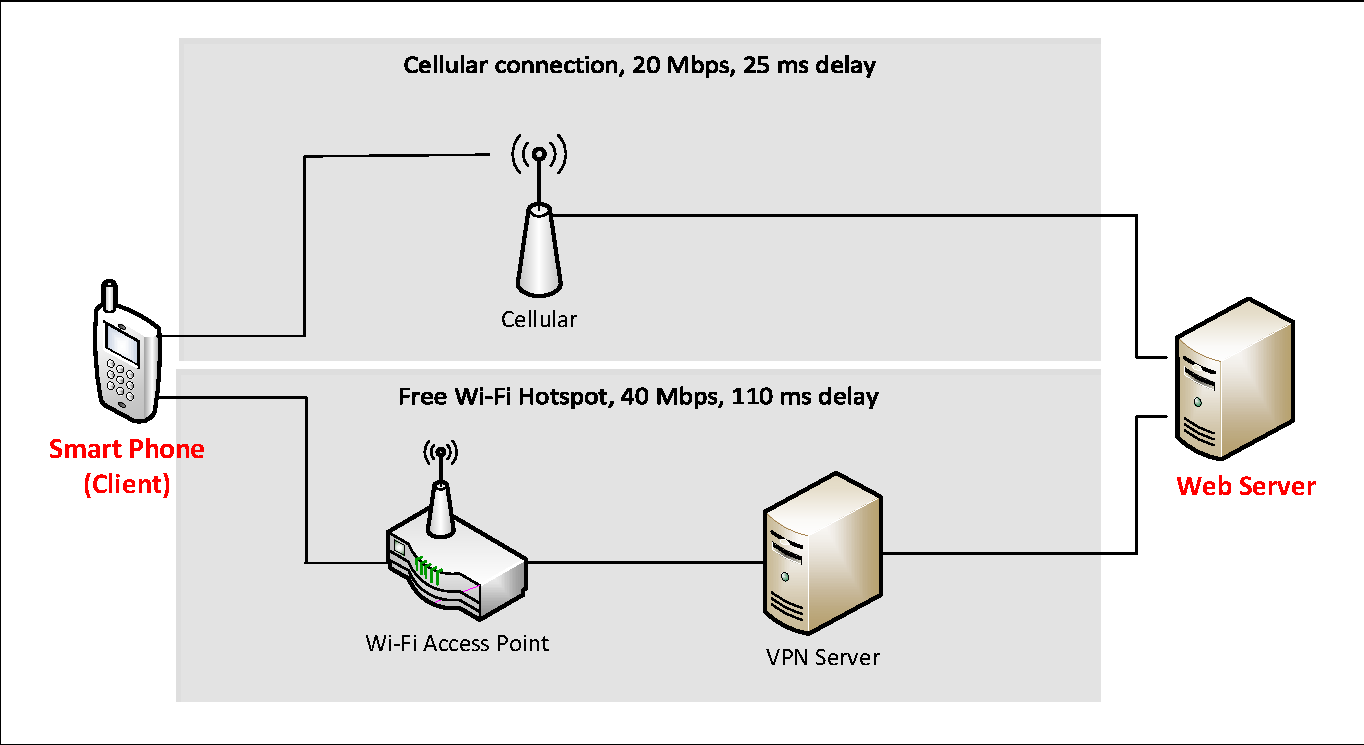
\includegraphics[width=0.9\textwidth]{eva1-scenario.pdf}
	\caption{Network scenario which is simulated in Evaluation A }
	\label{eva1-scenario}
\end{figure}

\begin{figure}
\centering
	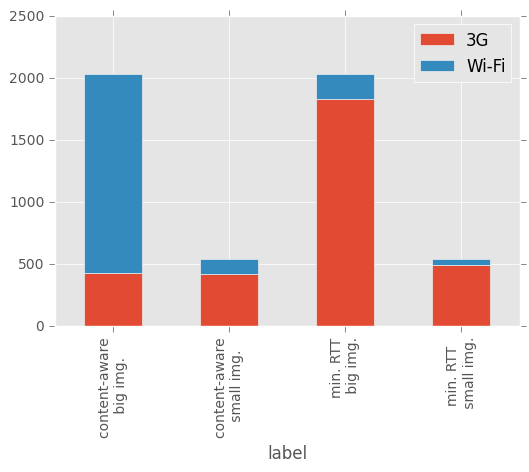
\includegraphics[width=0.45\textwidth]{eva1-rxbytes.png}
	\caption{Received bytes per interface for Evaluation A }
	\label{eva1-rxbytes}
\end{figure}

\begin{figure}
\centering
	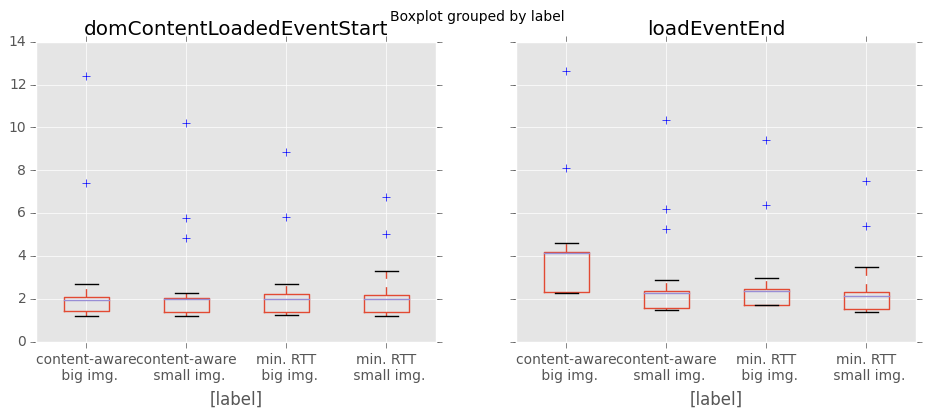
\includegraphics[width=0.9\textwidth]{eva1-loadtimes.png}
	\caption{Page load times for Evaluation A }
	\label{eva1-loadtimes}
\end{figure}


% simulated netw. with mininet
% - two hosts, two paths
% - path one (slow Wi-Fi hotspot, e.g. over vpn) - bw=50, delay=110
% - path two (LTE) - bw=50, delay=50
% server: nghttpd, modified for RBS socket options
% - hint: content type (document, style, script, image, other)
% scheduler: rbs
% - forTest: script 1: redundant for document+style
% - forTest: script 2: never transmit images on LTE
% baselines:
% - script 3: redundant scheduler (everything redundant)
% - linux mptcp default scheduler
% - single path tcp on Wi-Fi
% - single path tcp on LTE
% web site:
% - synthetic web site with:




% later ajax redundant
% oder images only one sbf


\subsection{Evaluation B }

%maybe redundant for ``important'' stuff?
% ...combination, switch dependent on RTT and LOSS -- maybe do this in a separate Eval C










%=====================================================================
\chapter{Conclusion}
%=====================================================================



\section{Outlook / Future Work}

%-------------------------------------------------------
%client side

The client (web browser) side of optimizations was mostly excluded from our considerations. 
% one might implement a mptcp protocol extension so the logic can sit mostly in browser OR webserver, and the other side is instructed what to do
% another way to generalize this could be definining a way for the web page/app to give the hints to the browser, which passes them on to the client mptcp scheduler
% -> the server scheduler implementation could send the corresponding mptcp frames with the same scheduling strategy as the request

% on the other hand, a different, quite simple approach could be taken on the browser side: send regular GET requests (maybe also POST with small body) as fast, latency critical strategy, while sending big POSTs (uploads) as latency uncritical strategy
% it might be possible to do a good heuristical approach here, without support from the browser, only in the mptcp scheduler

%-------------------------------------------------------
%more interfaces

% ***Extension to three or more interfaces

%-------------------------------------------------------
%automated web site analysis

% ***our work could be combined with :
Some optimizations rely on manually providing resource priorities and dependencies to the web server. Our work could be combined with automated algorithms to determine dependency graphs of web pages and user relevancy ratings of resources. Butkiewicz et al. \cite{klotski2015}

% - automated categorization of ressources/http requests

% - automated dependency graph

%Automatische Einstufung von Seitenbestandteilen (HTTP Requests) in Relevanz / User Utility
%-> nicht Thema der Arbeit, aber evtl. relevant f�r praktische Umsetzung

%Automatisches Aufbauen von Dependency Graphs


%-------------------------------------------------------
%real web server

% ***Porting to a ``real'' web server e.g. apache or nginx




%=====================================================================
% Bibliography
%=====================================================================


\nocite{*}
%\chapter{Bibliography}
%\bibliography{thesis-h2-mptcp}{}
\printbibliography




\end{document}
